%
% chapter.tex -- Topologie
%
% (c) 2025 Prof Dr Andreas Müller
%
\chapter{Topologie
\label{chapter:topologie}}
\kopflinks{Topologie}
%
% fig-torus.tex
%
% (c) 2025 Prof Dr Andreas Müller
%
\begin{figure}
\centering
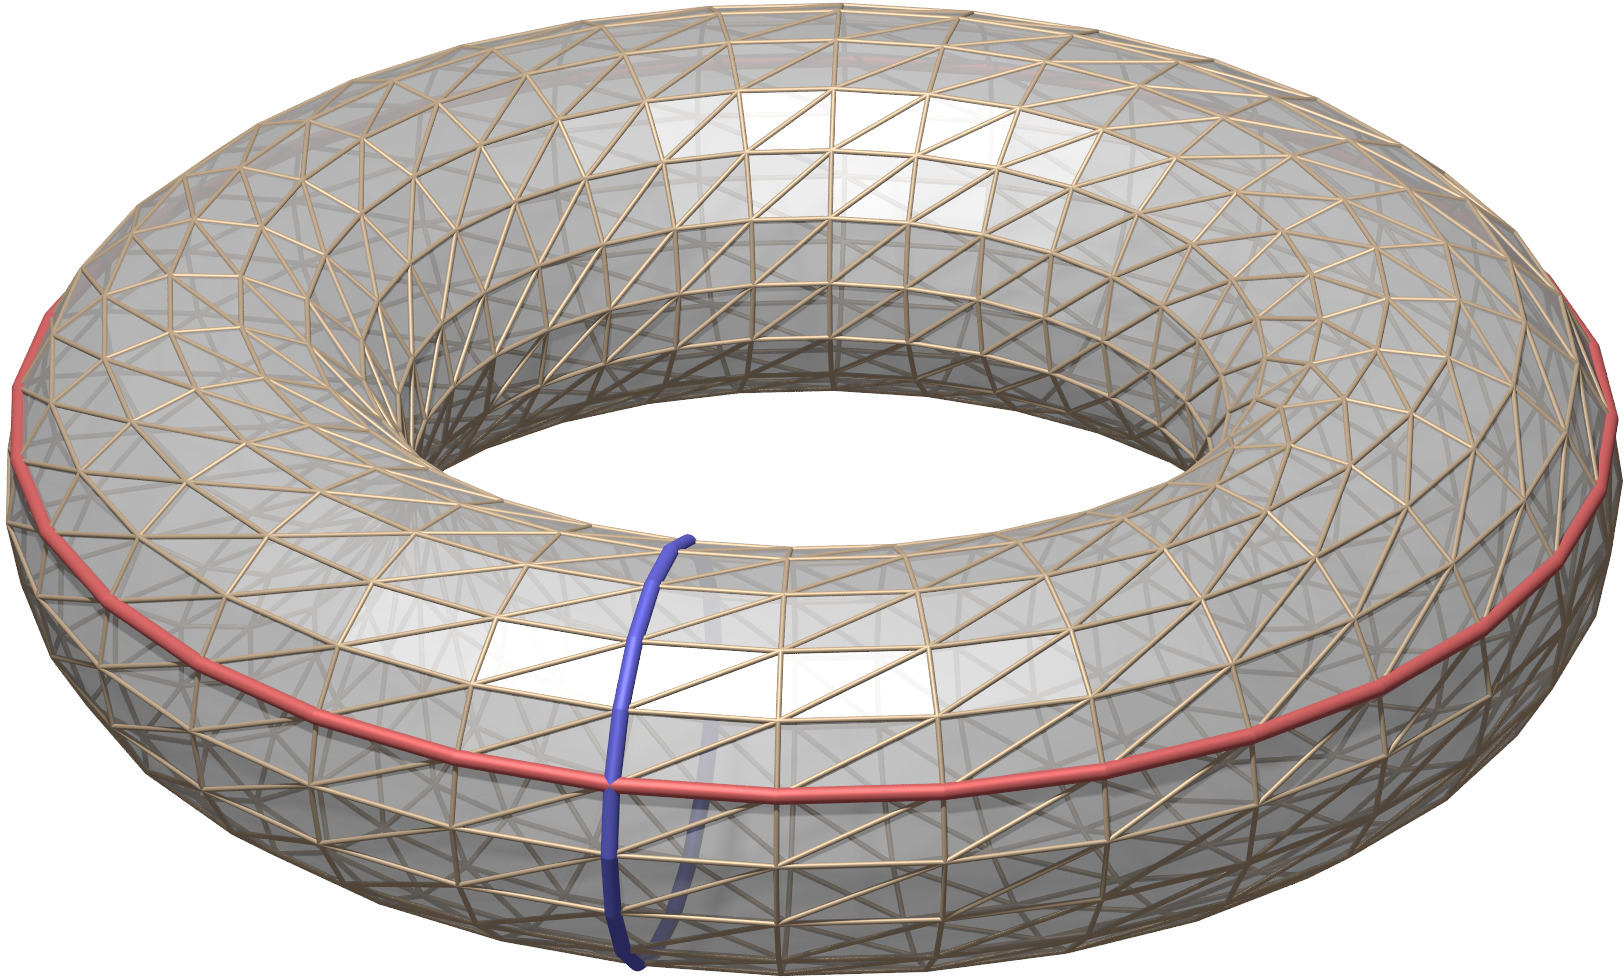
\includegraphics[width=\textwidth]{chapters/120-topologie/images/torus.jpg}
\caption{Triangulation eines Torus mit 576~Ecken, 1728~Kanten und
1152~Dreiecken.
Der Torus hat daher die Euler-Charakteristisk $0$.
\label{buch:topologie:intro:fig:torus}}
\end{figure}
%
%
% fig-sphaere.tex
%
% (c) 2025 Prof Dr Andreas Müller
%
\begin{figure}
\centering
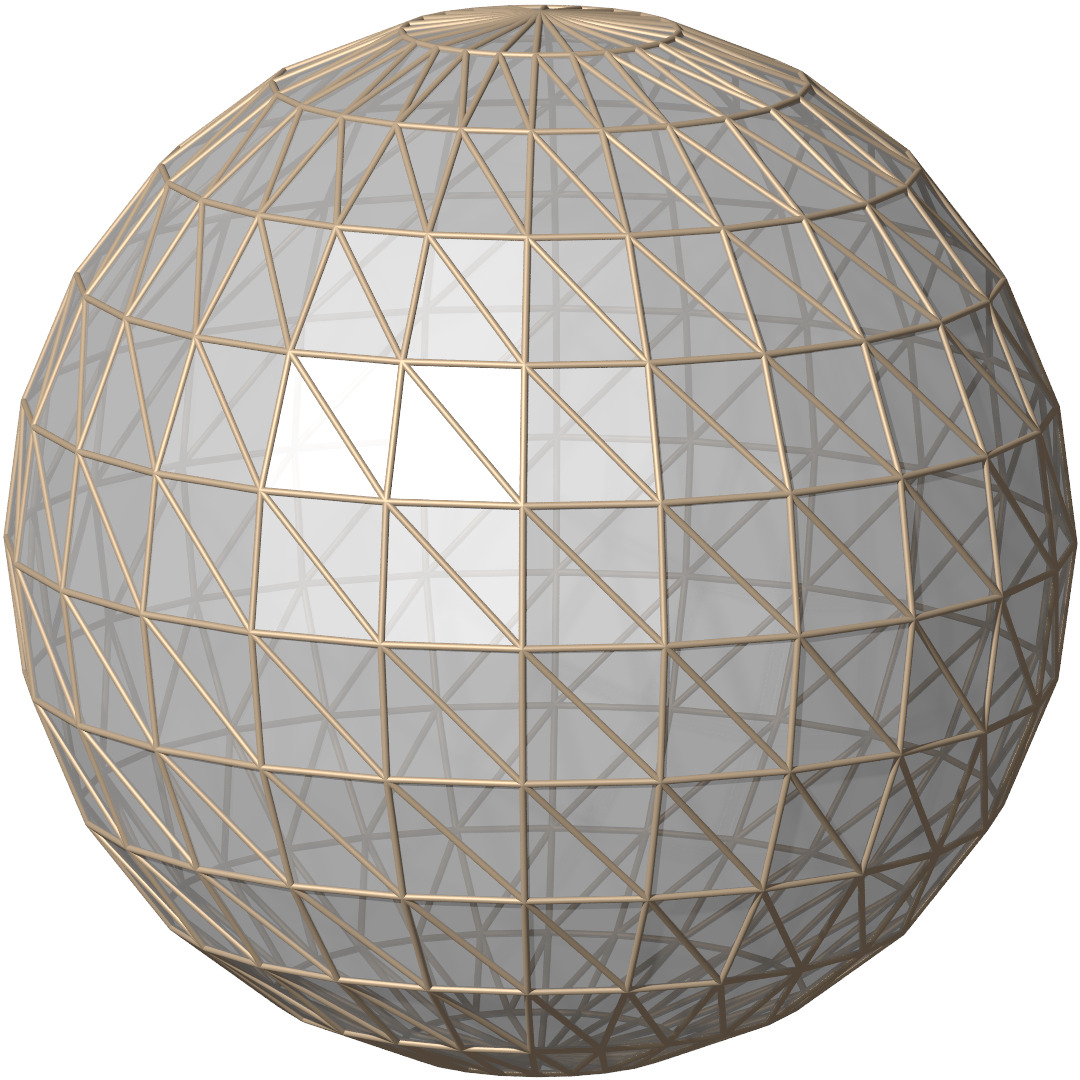
\includegraphics[width=0.6\textwidth]{chapters/120-topologie/images/sphaere.jpg}
\caption{Triangulation einer Kugel mit 266~Ecken, 792~Kanten und
528~Dreiecken.
Die Kugel hat daher die Euler-Charakteristisk $2$.
\index{Kugel}%
\index{Triangulation}%
\label{buch:topologie:intro:fig:sphere}}
\end{figure}
%
%
% table-polyeder.tex
%
% (c) 2025 Prof Dr Andreas Müller
%
\begin{table}
\centering
\begin{tabular}{l>{$}r<{$}>{$}r<{$}>{$}r<{$}>{$}r<{$}}
\hline
Polyeder          &\text{Ecken}&\text{Kanten}&\text{Flächen}&\chi(M)\\
\hline
Tetraeder         &           4&            6&             4&      2\\
Oktaeder          &           6&           12&             8&      2\\
Hexader (Würfel)  &           8&           12&             6&      2\\
Dodekaeder        &          20&           30&            12&      2\\
Ikosaeder         &          12&           30&            20&      2\\
\hline
Kugel             &         266&          792&           528&      2\\
Torus             &         576&         1728&          1152&      0\\
\hline
\end{tabular}
\caption{Die eulerschen Polyeder haben alle die Euler-Charakteristik $2$.
Während die Triangulation einer Kugel aus
\index{Euler-Charakteristik}%
\index{Tetraeder}%
\index{Oktaeder}%
\index{Hexaeder}%
\index{Würfel}%
\index{Dodekaeder}%
\index{Ikosaeder}%
Abbildung~\ref{buch:topologie:intro:fig:sphere} wie die Polyeder
Euler-Charakteristik $2$ hat, ergibt die Triangulation des Torus von
\index{Triangulation}%
Abbildung~\ref{buch:topologie:intro:fig:torus} jedoch
der Wert 0, der zum Ausdruck bringt, dass der Torus ein ``Loch''
\index{Torus}%
\index{Kugel}%
hat.
\label{buch:topologie:intro:table:eulercharakteristik}}
\end{table}
%

\noindent
Das Poincaré-Lemma ist der erste Hinweis darauf, dass die grossräumige
\index{Poincare-Lemma@Poincaré-Lemma}%
\index{Topologie}%
Gestalt einer Mannigfaltigkeit einen Einfluss darauf hat, ob sich eine
Differentialgleichung lösen lässt.
Es sagt nämlich, dass es auf einer zusammenziehbaren Mannigfaltigkeit
immer eine Lösung der Gleichung $d\alpha = 0$ im Raum der $p$-Formen
gibt.
Die Kohomologietheorie vertieft diese Idee und definiert eine Familie
\index{Kohomologie}%
von Vektorräumen, deren Dimension angibt, wieviele in noch zu definierendem
Sinn wesentlich verschiedene Lösungen eine solche Gleichung haben kann.
Diese Dimensionszahlen geben wesentliche Informationen über die grossräumige
Gestalt der Mannigfaltigkeit.

Auf Leonhard Euler geht die Beobachtung zurück, dass für ein beliebiges
\index{Euler, Leonhard}%
geschlossenes Polyeder ohne Löcher im Raum immer
\begin{equation}
\#\{\text{Ecken}\}
-
\#\{\text{Kanten}\}
+
\#\{\text{Flächen}\}
=
E-K+F
=
2
\label{buch:topologie:eqn:eulerpolyeder}
\end{equation}
gilt.
Da sich eine beliebige zweidimensionale Mannigfaltigkeit triangulieren
lässt, kann diese Zahl auch für eine Triangulierung berechnet werden.
Es stellt sich heraus, dass 
die Zahl \eqref{buch:topologie:eqn:eulerpolyeder}
nicht von der Triangulierung abhängt und sich auch aus den Dimensionszahlen
der Kohomologievektorräume berechnen lässt.
Sie heisst heute die Euler-Charakteristik $\chi(M)$ einer Mannigfaltigkeit.
Tabelle~\ref{buch:topologie:intro:table:eulercharakteristik} enthält
eine Zusammenstellung der Euler-Charakteristiken der eulerschen Polyeder
sowie von Triangulationen von Torus und Kugel.
\index{Kugel}%
\index{Torus}%

Das Gebiet der algebraischen Topologie befasst sich genau mit dieser Art
\index{Topologie!algebraische}
der Beschreibung der ``Gestalt'' von topologischen Räumen.
Für Mannigfaltigkeiten stellt sie einen besonders vielfältigen
Werkzeugkasten bereit, der solche Fragestellungen sowohl mit
kombinatorischen wie auch mit analytischen Aspekten einer Mannigfaltigkeit
verbinden kann.
Ziel dieses Kapitels ist, einen Ausblick auf die wichtigsten Ideen
dieser reichhaltigen Theorie zu geben.

%
% Simpliziale Homologie
%
\section{Simpliziale Homologie
\label{buch:topologie:section:simplex}}
\kopfrechts{Simpliziale Homologie}%
Die von Leonhard Euler entdeckte kombinatorische Eigenschaft der platonischen
\index{Euler, Leonhard}%
Körper lässt sich auf beliebige triangulierte Körper und sogar
\index{platonische Korper@platonischer Körper}%
auf Mannigfaltigkeiten höherer Dimension ausdehnen.
Die Vorgehensweise und die wichtigsten Eigenschaften sollen in den
folgenden Abschnitten skizziert werden.

%
% Zellenkomplexe
%
\subsection{Zellenkomplexe}
Eine Triangulation einer Fläche zerlegt die Fläche in Dreiecke,
Kanten und Punkte.
\index{Triangulation}%
Dabei müssen Ecken und Kanten von benachbarten Dreiecken aufeinander
fallen.
Es ist zum Beispiel nicht zulässig, dass eine Ecke eines Dreiecks
auf einen inneren Punkt einer Kante eines Nachbardreiecks fällt.
Der Begriff des Zellenkomplexes verallgemeinert die Idee
der Triangulation und erlaubt, damit zu rechnen.
\index{Triangulation}%
\index{Zellenkomplex}%

%
% Simplizes
%
\subsubsection{Simplizes}
Punkte, Kanten und Dreieck sind die vertraute Spezialfälle des allgemeinen
\index{Punkt!als $0$-Simplex}%
\index{Kante, als $1$-Simplex}%
\index{Dreieck, als $2$-Simplex}%
Konzeptes eines Simplex.
%
% fig-simplex.tex
%
% (c) 2025 Prof Dr Andreas Müller
%
\begin{figure}
\centering
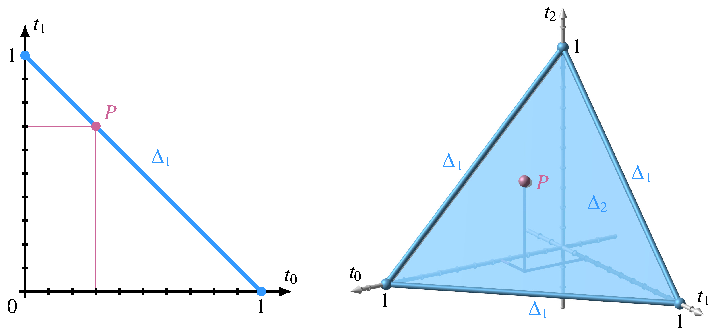
\includegraphics{chapters/120-topologie/images/simplex.pdf}
\caption{Ein- und zweidimensionale Simplizes als Punktmengen in
$\mathbb{R}^{k+1}$ für $k=1,2$.
Die Schnittmengen von $\Delta_2$ mit den Koordinatenebenen bilden
jeweils ein 1-Simplex.
\label{buch:topologie:simplex:fig:simplex}}
\end{figure}
%

\begin{definition}[Simplex]
\index{Simplex}%
Ein \emph{$n$-dimensionales Simplex} ist die Menge
\index{Simplex}%
\index{n-Simplex@$n$-Simplex}%
\[
\Delta_n
=
\{
(t_0,\dots,t_n)
\subset
[0,1]^{n+1}
\mid
t_0+\dots+t_n=1
\}.
\]
\end{definition}

Im Falle $n=0$ besteht $\Delta_0$ nur aus der Zahl $1$.
$\Delta_1$ besteht aus Paaren $(t_0,t_1)$ mit $t_0+t_1=1$, die
als die Strecke zwischen $(1,0)$ und $(0,1)$ visualisiert
werden (Abbildung~\ref{buch:topologie:simplex:fig:simplex} links).
Ebenso besteht die Menge $\Delta_2$ aus den Punkten der Ebene mit
der Gleichung $t_1+t_2+t_3=1$ im postiven Oktanten eines
dreidimensionalen kartesischen Koordinatensystems mit Koordinaten
$t_1$, $t_2$ und $t_3$
(Abbildung~\ref{buch:topologie:simplex:fig:simplex} rechts).

In der Teilmenge
\[
\Delta_{n,i}
=
\{
(t_0,\dots,t_n)
\subset
[0,1]^{n+1}
\mid
t_0+\dots+t_n=1
\wedge
t_i=0
\}
\subset
\Delta_n
\]
sind $n+1$-Tupel, deren $i$-Koordinate verschwindet.
Die Mengen $\Delta_{n,i}$ heissen die \emph{Seitenflächen}
\index{Seitenflache@Seitenfläche}%
des Simplex $\Delta_n$.

Für die verbleibenden Koordinaten gilt wegen $t_i=0$ ebenfalls
\[
t_0+\dots+t_i+\dots+t_n
=
t_0+\dots+\widehat{t_i}+\dots+t_n
=
1,
\]
wobei der Hut bedeutet, dass dieser Term weggelassen wird.
Man kann die Menge also durch die Abbildung
\[
\iota_i
\colon
\Delta_{n-1}
\to
\Delta_{n,i}
:
(t_0,\dots,t_{n-1})
\mapsto
(t_0,\dots,0,\dots,t_{n-1})
\]
parametrisieren.
Die Abbildung $\iota_i$ ist bijektiv, stetig und die Umkehrung ist
ebenfalls stetig.
Die Seitenflächen $\Delta_{n,i}$ sind also Simplizes kleinerer 
Dimension.

Zwei Seitenflächen eines Simplex stossen in einer Menge zusammen,
die ein Simplex der Dimension $n-2$ ist.
Die gemeinsamen Punkte der beiden Seitenflächen $\Delta_{n,i}$ und
$\Delta_{n,k}$ bilden die Menge
\[
\Delta_{n,ik}
=
\{
(t_0,\dots,t_n)
\mid
t_0+\dots+t_n=1
\wedge
t_i=0
\wedge
t_k=0
\},
\]
die sich nach dem gleichen Muster wie die Seitenfläche mit der Menge
$\Delta_{n-2}$ identifizieren lässt.

\begin{definition}[Zellenkomplex]
\index{Zellenkomplex}%
Ein \emph{Zellenkomplex} ist ein topologischer Raum, der durch
Zusammenfügen von endlich vielen Simplizes entlang von Untersimplizes
kleinerer Dimension entsteht.
\index{Dimension}%
Die \emph{Dimension} eines Zellenkomplexes ist die höchste Dimension
der Simplizes, aus denen er besteht.
\end{definition}

Ein Zellenkomplex der Dimension $n$ setzt sich also aus maximal
$n$-dimensionalen Simplizes zusammen, die Seitenflächen oder
Simplizes noch kleinerer Dimension gemeinsam haben können.

%
% Euler-Charakteristik eines Zellenkomplexes
%
\subsubsection{Euler-Charakteristik eines Zellenkomplexes}
Eulers Entdeckung bezog sich auf Polyeder, die sich natürlich nur
aus Ecken, Kanten und Flächen, also Simplizes der Dimension 0, 1
bzw.~2.
Bezeichnen wir die Anzahl der $k$-dimensionalen Simplizes mit $t_k$,
dann wird die von Euler berachtete Summe 
\begin{align*}
E - K + K
&=
t_0
-
t_1
+
t_2,
\intertext{die wir auch}
&=
\sum_{k=0}^2 (-1)^kt_k
\end{align*}
schreiben können.
Diese Schreibweise lässt sich leicht auf beliebige Dimension
verallgemeinern.

\begin{definition}[Euler-Charakteristik]
Sei $S$ ein $n$-dimensionaler Zellenkomplex in dem
genau $k_i$ Simplizes der Dimension $i$ vorkommen.
Dann ist die Summe
\[
\chi(S)
=
k_0 - k_1 + \dots + (-1)^n t_n
=
\sum_{i=0}^n (-1)^i k_i
\]
die \emph{Euler-Charakteristik} von $S$.
\index{Euler-Charakteristik}%
\index{Euler-Charakteristik!eines Zellenkomplexes}%
\end{definition}

%
% Verfeinerung eines Zellenkomplexes
%
\subsubsection{Verfeinerung eines Zellenkomplexes}
Die Definition der Euler-Charakteristik hängt von der Triangulation ab.
Wir müssen daher zeigen, dass eine Verfeinerung eines Zellenkomplexes die
Euler-Charakteristik nicht ändert.
Statt eines vollständigen Beweises dieser Eigenschaft zeigen wir anhand
einiger illustrativer Beispiele, was sich bei der Verfeinerung
abspielt.
%
% fig-unterteilung.tex
%
% (c) 2025 Prof Dr Andreas Müller
%
\begin{figure}
\centering
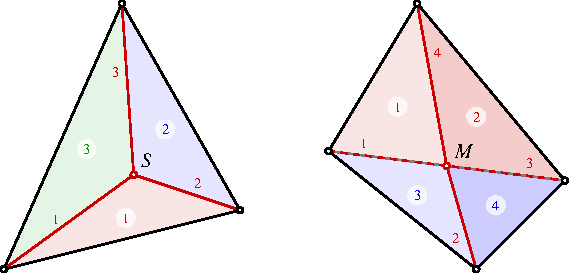
\includegraphics{chapters/120-topologie/images/unterteilung.pdf}
\caption{Links: Bei der Unterteilung eines einzelnen Dreiecks durch einen
inneren Punkt $S$ entstehen drei Dreieck ($2$ mehr also vor der Unterteilung)
und 3 neue Kanten.
Rechts: Bei der Unterteilung der Kante $AB$ durch den Punkt $M$ werden
\index{Unterteilung}%
beide Nachbardreiecke (rot und blau) in jeweils zwei Dreiecke
($2$ mehr als vor der Unterteilung)$ zerlegt.
Ausserdem entstehen drei zusätzliche Kanten.
In allen Fällen ändert sich die Euler-Charakteristik nicht.
\label{buch:topologie:eulercharakteristik:fig:unterteilung}}
\end{figure}
%

Wir beginnen mit einem zweidimensionalen Zellenkomplex
und betrachten ein einzelnes Dreieck.
Der Zellenkomplex kann verfeinert werden, indem im Inneren des
Dreiecks ein weiterer Punkt hinzugefügt wird
(Abbildung~\ref{buch:topologie:eulercharakteristik:fig:unterteilung} links).
Neue Kanten vom neuen Punkt zu den Ecken des Dreiecks ergeben die
verfeinerte Triangulation.
Die Triangulation bekommt also eine zusätzliche Ecke, drei zusätzliche
Kanten und aus einem Dreieck werden drei, also zwei zusätzliche Dreiecke.
Für die Euler-Charakteristik bekommen wir daher
\[
(E+1) - (K+3) - (F+2)
=
E-K+F+(\underbrace{1-3+2}_{\displaystyle=0})
=
E-K+F,
\]
die Euler-Charakteristik ändert also nicht.

Unterteilt man eine Kante mit einem neuen Punkt, dann müssen auch
die angrenzenden beiden Dreiecke mit einer Kante zur gegenüberliegenden
Ecke neu unterteilt werden
(Abbildung~\ref{buch:topologie:eulercharakteristik:fig:unterteilung} rechts).
Die Anzahl der Ecken vergrössert sich um eins.
Aus der ursprünglichen Kante werden zwei und es kommen zwei neue Kanten
dazu.
Die Anzahl der Dreiecke wächst um zwei.
Die Euler-Charakteristik ist neu
\begin{align*}
(E+1) - (K+3) - (F+2)
=
E-K+F +(\underbrace{1-3+2}_{\displaystyle=0})
=
E-K+F,
\end{align*}
sie verändert sich also auch bei Unterteilung einer Kante nicht.

In drei Dimensionen wird die Unterteilung etwas komplizierter.
Ein zusätzlicher innerer Punkt in einem Tetraeder zerlegt
es in vier Tetraeder mit dem neuen Punkt als Spitze und den
Seitenflächen des ursprünglichen Tetraeders als Grundfläche.
Für jede ursprüngliche Kante entsteht eine neue Fläche und
für jede ursprüngliche Ecke eine neue Kante.
Die Euler-Charakteristik wird daher zu
\begin{align*}
(E+1) - (K+4) + (F+6) - (V+3)
&=
E-K+F-V
+
(\underbrace{1-4+6-3}_{\displaystyle=0})
\\
&=
E-K+F-V
=
\chi(M),
\end{align*}
bleibt daher unverändert.

Unterteilt man eine Dreiecksfläche durch einen inneren Punkt,
müssen auch die beiden benachbarten Tetraeder unterteilt werden.
Dabei entstehen fünf neue Kanten, sechs neue Flächen und vier
neue Tetraeder.
Die neue Euler-Charakteristik ist daher
\begin{align*}
(E+1) - (K+5) + (F+8) - (V+4)
&=
E-K+F-V
+(\underbrace{1-5+8-4}_{\displaystyle=0})
\\
&=
E-K+F-V
=
\chi(M),
\end{align*}
ebenfalls unverändert.

Schliesslich betrachten wir den Fall der Unterteilung einer Kante,
die $n$ Tetraedern gemeinsam ist, mit $f$ Seitenflächen, die sich
in der Kante treffen.
Durch die Unterteilung wird aus jeder Seitenfläche zu zweien
mit einer zusätzlichen Kante.
Zusätzlich entsteht in jedem ursprünglichen Tetraeder ein zusätzliches
Dreieck mit der gegenüberliegenden Kante als Basis und der neuen
Ecke als Spitze.
Die Zahl der Tetraeder erhöht sich ebenfalls um $n$.
Die neue Euler-Charakteristik ist
\begin{align*}
(E+1)
-
(K+1+f)
+
(F+f+n)
-
(V+n)
&=
E-K+F-V + (\underbrace{1-1-f+f+n-n}_{\displaystyle=0})
\\
&=
E-K+F-V
=
\chi(M),
\end{align*}
wieder unverändert.

Dieselbe Art von Rechnung lässt sich auch für Simplizes beliebig hoher
Dimension durchführen.
Ohne auf den detaillierten Beweis einzugehen, können wir schliessen,
dass die Euler-Charakteristik eine Grösse ist, die nicht von der Unterteilung
des Körpers in Simplizes abhängt.
Die Euler-Charakteristik ist also eine topologische Invariante.

%
% Rand
%
\subsubsection{Rand}
%
% fig-rand.tex
%
% (c) 2025 Prof Dr Andreas Müller
%
\begin{figure}
\centering
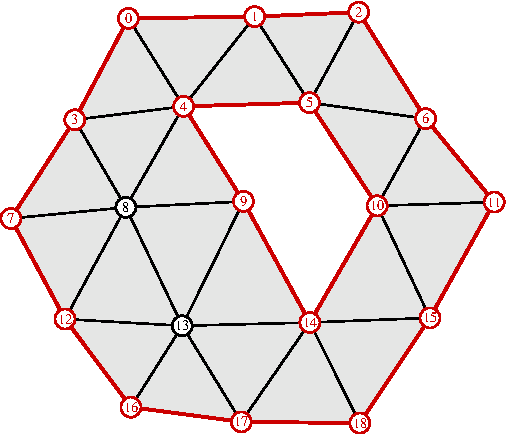
\includegraphics{chapters/120-topologie/images/rand.pdf}
\caption{Rand eines zweidimensionalen simplizialen Komplexes.
\index{Rand}
Die schwarzen Kanten sind innere Kanten und gehören nicht zum Rand.
Nur Kanten, die zu nur einem 2-Simplex gehören, tragen zum Rand bei.
\label{buch:topologie:homologie:fig:rand}}
\end{figure}
%
Ein $n$-Simplex mit den Ecken $p_0\dots p_n$ besteht aus den $(n-1)$-Simplizes,
denen genau eine Ecke fehlt.
Wenn aber zwei $n$-Simplizes entlang eines gemeinsamen $(n-1)$-Simplex
zusammenstossen, dann möchte man dieses nicht als Teil des Randes
des Zellenkomplexes betrachten.
Abbildung~\ref{buch:topologie:homologie:fig:rand} illustriert das Problem.
Die rote eingezeichneten Kanten bilden zusammen den Rand.
Die schwarzen Kanten sind innere Kanten, die jeweils zwei Dreiecken 
gemeinsam sind und nicht zum Rand gezählt werden dürfen.


%
% Homologie
%
\subsection{Kettenkomplexe
\label{buch:topologie:subsection:kettenkomplexe}}
In der linearen Algebra lernt man, dass man ein elektrisches
Netzwerk mit Hilfe von Matrizen beschreiben kann
\cite[Abschnitt~2.A]{buch:linalg}.
Die zum Beispiel für die kirchhoffschen Regeln benötigten Zyklen
im Netzwerk werden beschrieben als Vektoren, deren Komponenten angeben,
welche Kanten zum Zyklus gehören.
Zur Verifikation, dass es sich um einen Zyklus handelt, erfolgt dann
durch Anwendung einer Matrix $\partial$, welche den Endpunkten der
Kanten Zahlen $\pm 1$ zuweist.
Ein Zyklus liegt vor, wenn in der Summe keine Ecke übrig bleibt.
Die Diskussion des Randes am Ende des vorangegangenen Abschnittes
zeigt, dass die Idee des Rechnens mit Ecken mit rellen Koeffizienten 
auf Simplizes beliebiger Dimension ausgeweitet werden muss.
Dabei entsteht das algebraische Konzept eines Kettenkomplexes.

%
% Vektorraum der Simplizes
%
\subsubsection{Vektorraum der Simplizes}
Der Rand eines Simplexes ist nicht ein einzelnes Simplex, sondern
eine Menge von Simplizes.
Genau genommen müssen wir ausserdem auch noch die Orientierung eines
Simplexes berücksichtigen.
Ein zweidimensionales Simplex mit den Ecken $ABC$ hat als Rand
die drei Simplizes $AB$, $BC$ und $AC$, aber das letzte wird in
entgegengesetzter Richtung durchlaufen.

\begin{definition}
Sei $S$ ein $n$-dimensionaler Zellenkomplex.
Für jedes $k$, $0\le k\le n$ ist $C_k$ der reelle Vektorraum aufgespannt
von den Simplizes von $S$.
Die Elemente $c\in C_k$ sind Linearkombinationen von $k$-dimensionalen
Simplizes.
Sie werden auch $k$-dimensionale \emph{Ketten} genannt.
\index{Kette}%
\end{definition}

\begin{beispiel}
\label{buch:topologie:eulercharakteristik:bsp:dreieck}
Wir betrachten den Zellenkomplex, der aus nur einem Dreieck
$\triangle ABC$ besteht.
Die $0$-dimensionalen Simplizes sind die Ecken $A$, $B$ und $C$, 
die eindimensionalen Simplizes sind die Kanten $AB$, $BC$ und $AC$.
Daher sind die Vektorräume $C_k$ gegeben durch
\begin{align*}
C_0 &= \{ x_A A + x_B B + x_C C\mid x_A, x_B, x_C\in\mathbb{R}\}
&
\dim C_0 &= 3
\\
C_1 &= \{ x_{AB} AB + x_{BC} BC + x_{AC} AC\mid x_{AB}, x_{BC}, x_{AC} \in\mathbb{R}\}
&
\dim C_1 &= 3
\\
C_2 &= \{ x_{ABC} ABC\mid x_{ABC}\in\mathbb{R}\}
&
\dim C_2 &= 1.
\qedhere
\end{align*}
\end{beispiel}

%
% Randoperator
%
\subsubsection{Randoperator}
Da wir jetzt beliebige Simplizes linear kombinieren können, können
wir auch den Rand eines Simplex als Linearkombination von
niedrigerdimensionaler Simplizes ausdrücken.

\begin{definition}[Randoperator]
Der $k$-dimensionale Randoperator ist die lineare Abbildung
\[
\partial_k
\colon
C_k \to C_{k-1}
:
P_0\dots P_k
\mapsto
\sum_{i=0}^k
(-1)^i
P_0\dots\widehat{P_i}\dots P_k.
\]
\index{Randoperator}%
\end{definition}

\begin{beispiel}
\label{buch:topologie:eulercharakteristik:bsp:dreieckrand}
Das Beispiel~\ref{buch:topologie:eulercharakteristik:bsp:dreieck}
konstruiert die Vektorräume $C_k$ für ein Dreieck.
\index{Tetraeder}%
Der $0$-dimensionale Randoperator $\partial_0$ ist der Null-Operator.
In höheren Dimension sind Randoperatoren gegeben durch
\begin{align*}
\partial_1 AB &= -B + A &&&&\\
\partial_1 BC &= -C + B &
&\Rightarrow
&\partial_1&=\smash{\begin{pmatrix*}[r]
 1 &  0 &  1 \\
-1 &  1 &  0 \\
 0 & -1 & -1
\end{pmatrix*}}
\\
\partial_1 AC &= -C + A \\
\partial_2 ABC &= AB - AC + BC&&\Rightarrow&\partial_2&=\begin{pmatrix*}[r]1\\1\\-1\end{pmatrix*}
\end{align*}
Als Basis für die Matrixdarstellung der Randoperatoren wird die
Reihenfolge der $k$-Simplizes im
Beispiel~\ref{buch:topologie:eulercharakteristik:bsp:dreieck}
verwendet.

Die gefundenen Randoperatoren wirken zwischen den Vektorräumen $C_k$
wie im Diagramm.
\[
 0                  \xleftarrow{\qquad\clap{$\partial_0=0$}\qquad}
C_0 = \mathbb{R}    \xleftarrow{\qquad\clap{$\partial_1$}\qquad}
C_1 = \mathbb{R}^3  \xleftarrow{\qquad\clap{$\partial_2$}\qquad}
C_2 = \mathbb{R}    \xleftarrow{\qquad\clap{$\partial_3=0$}\qquad}
 0.
\]
Der Rand des Dreiecks ist eine geschlossene Kurve, man erwartet
also, dass der Rand des Randes $0$ ist.
Tatsächlich ist das Produkt der Matrizen 
\begin{align*}
\partial_1\circ\partial_2
=
\begin{pmatrix*}[r]
 1 &  0 &  1 \\
-1 &  1 &  0 \\
 0 & -1 & -1
\end{pmatrix*}
\begin{pmatrix*}[r] 1 \\ 1 \\ -1 \end{pmatrix*}
&=
\begin{pmatrix}0\\0\\0\end{pmatrix}.
\end{align*}
wie erwartet.
\end{beispiel}

\begin{satz}
Der Rand eines Randes verschwindet, $\partial_{k-1}\circ\partial_k=0$.
\end{satz}

\begin{proof}
Da der Randoperator linear ist, muss die Behauptung nur auf $k$-dimensionalen
Simplizes verifiziert werden.
Sei also $\sigma=P_0\dots P_k$ ein $k$-dimensionales Simplex.
Der Randoperator ergibt
\[
\partial_k\sigma
=
\sum_{i=0}^k
(-1)^i P_0\dots\widehat{P_i}\dots P_k.
\]
Die Summanden sind $k-1$-dimensionale Simplizes, deren Rand wir jetzt
zusätzlich ausrechnen müssen.
Dabei müssen erneut Punkte $P_j$ weggelassen und mit einem Vorzeichen versehen
werden.
Da das Vorzeichen von der Position und nicht vom Index abhängt, unterscheiden
wird die Fälle $j<i$ und $j>i$:
\begin{align*}
\partial_{k-1}\partial_k \sigma
&=
\sum_{i=0}^k (-1)^i \partial_{k-1} P_0\dots \widehat{P_i}\dots P_k
\\
&=
\sum_{i=0}^k
\biggl(
\sum_{j=0}^{i-1}
(-1)^{i+j}P_0\dots\widehat{P_j}\dots \widehat{P_i}\dots P_k
+
\sum_{j=i+1}^{k}
(-1)^{i+j+1}P_0\dots\widehat{P_i}\dots \widehat{P_j}\dots P_k
\biggr)
\\
&=
\sum_{j<i}
(-1)^{i+j}P_0\dots\widehat{P_j}\dots \widehat{P_i}\dots P_k
+
\sum_{i<j}
(-1)^{i+j+1}P_0\dots\widehat{P_i}\dots \widehat{P_j}\dots P_k.
\intertext{Vertauschen wir die Namen der Summationsvariablen in der
zweiten Summe und verwandeln wird den Summanden $+1$ im Exponenten
in ein Vorzeichen vor der Summe, entsteht}
&=
\sum_{j<i}
(-1)^{i+j}P_0\dots\widehat{P_j}\dots \widehat{P_i}\dots P_k
-
\sum_{j<i}
(-1)^{i+j}P_0\dots\widehat{P_j}\dots \widehat{P_i}\dots P_k.
\end{align*}
Die beiden Summen heben sich weg, was die Behauptung beweist.
\end{proof}

%
% Kettenkomplex
%
\subsubsection{Kettenkomplex}
Der Randoperator $\partial_k$ ist eine lineare Operation, die den Grad 
erniedrigt.
Ausserdem gilt, dass der iterierte Randoperator verschwindet.
Diese algebraische Struktur tritt auch in anderen Zusammenhängen
auf und verdient daher einen eigenen Namen, der in der folgenden
Definition eingeführt wird.

\begin{definition}[Kettenkomplex]
Eine Folge von Vektorräumen $C_k$ und linearen Abbildungen
$\partial_k\colon C_k\to C_{k+1}$
mit der Eigenschaft $\partial_{k-1}\circ\partial_k=0$ heisst
ein \emph{Kettenkomplex}.
\index{Kettenkomplex}%
Kettenkomplexe werden manchmal auch $(C_*,\partial_*)$ notiert.
\end{definition}

Ein Kettenkomplex $(C_*,\partial_*)$ kann daher auch als Diagramm
\begin{equation}
\dots
\xleftarrow{\;\quad\clap{$\partial_{k-2}$}\quad\;}
C_{k-2}
\xleftarrow{\;\quad\clap{$\partial_{k-1}$}\quad\;}
C_{k-1}
\xleftarrow{\;\quad\clap{$\partial_{k}$}\quad\;}
C_k
\xleftarrow{\;\quad\clap{$\partial_{k+1}$}\quad\;}
C_{k+1}
\xleftarrow{\;\quad\clap{$\partial_{k+2}$}\quad\;}
\dots
\label{buch:topologie:simplex:eqn:kettenkomplex}
\end{equation}
von linearen Abbildung geschrieben werden.
Die Forderung, dass die Verkettung $\partial_{k-1}\circ\partial_k=0$
ist, ist gleichbedeutend mit der Forderung, dass das Bild von $\partial_k$
im Kern von $\partial_{k+1}$ enthalten ist, oder
$\operatorname{im}\partial_k \subset \ker\partial_{k-1}$.
Der Kern von $\partial_{k-1}$ kann aber durchaus grösser sein, es kann
also Elemente $c_{k-1}\in C_{k-1}$ geben mit $\partial_{k-1} c_{k-1}=0$,
für die es kein $c_k\in C_k$ gibt $c_{k-1}=\partial_kc_k$.

\begin{definition}[exakte Folge]
Eine Folge der Form
\eqref{buch:topologie:simplex:eqn:kettenkomplex}
heisst \emph{exakt} an der Stelle $k$, wenn
$\ker\partial_{k} = \operatorname{im}\partial_{k+1}$
gilt.
\end{definition}

\begin{beispiel}
\label{buch:topologie:eulercharakteristik:bsp:dreieckkomplexe}
Für das Dreieck $\triangle ABC$ wurden die Randoperatoren in
Beispiel~\ref{buch:topologie:eulercharakteristik:bsp:dreieckrand}
bereits berechnet.
$\partial_1$ ist eine $3\times 3$-Matrix mit Rang~2, somit ist
\begin{align*}
\dim C_0 &= 3 &
\operatorname{rank} \partial_0 &= 0&
&\Rightarrow&
\dim \operatorname{im}\partial_0 &= 0 &
\dim \ker\partial_0 &= 3
\\
\dim C_1 &= 3 &
\operatorname{rank} \partial_1 &= 2&
&\Rightarrow&
\dim \operatorname{im}\partial_1 &= 2 &
\dim \ker\partial_1 &= {\color{darkred}1}
\\
\dim C_2 &= 1 &
\operatorname{rank} \partial_2 &= 1&
&\Rightarrow&
\dim \operatorname{im}\partial_2 &= {\color{darkred}1} &
\dim \ker\partial_2 &= 0.
\end{align*}
Die beiden roten Zahlen zeigen, dass die Folge an der Stelle $k=1$
exakt ist.

Entfernt man das 2-Simplex $ABC$ aus dem Zellenkomplex, entsteht
ein nur noch eindimensionaler Zellenkomplex.
\begin{align*}
\dim C_0 &= 3 &
\operatorname{rank} \partial_0 &= 0&
&\Rightarrow&
\dim \operatorname{im}\partial_0 &= 0 &
\dim \ker\partial_0 &= 3
\\
\dim C_1 &= 3 &
\operatorname{rank} \partial_0 &= 2&
&\Rightarrow&
\dim \operatorname{im}\partial_1 &= 2 &
\dim \ker\partial_1 &= {\color{darkred}1}
\\
\dim C_2 &= 0 &
\operatorname{rank} \partial_0 &= 0&
&\Rightarrow&
\dim \operatorname{im}\partial_2 &= {\color{darkred}0} &
\dim \ker\partial_2 &= 0.
\end{align*}
Dieser Zellenkomplex ist also nicht mehr exakt an der Stelle $k=1$.
\end{beispiel}

Von besonderem Interesse sind als Kettenkomplexe, die \emph{nicht}
exakt sind.
Die Kettenkomplexe, die aus einem Zellenkomplex abgeleitet
werden, sind oft von dieser Art.
Das Beispiel~\ref{buch:topologie:eulercharakteristik:bsp:dreieckkomplexe}
zeigt, dass ``Löcher'' in einem Zellenkomplex die Exaktheit an einer 
Stelle zerstören können.
Der Begriff der Homologie dient dazu, die Nichtexaktheit zu messen und
damit mit algebraischen Mitteln topologische Information des Zellenkomplexes
zu extrahieren.

%
% Homologie
%
\subsection{Homologie
\label{buch:topologie:simplex:subsection:homologie}}
Der Kettenkomplex zu einem Zellenkomplex ermöglicht, mit Simplizes zu rechnen.
Die Bestimmung des Randes ist eine rein algebraische Operation
in einem Vektorraum geworden.
Damit wird es aber auch einfacher, mit speziellen Teilkomplexen
zu arbeiten, zum Beispiel solchen, die keinen Rand haben, oder solchen,
die als Rand eines Teilkomplexes entstanden sind.

%
% Zyklen und Ränder
%
\subsubsection{Zyklen und Ränder}
Der Randoperator ist ein linearer Operator und wird daher wesentlich
durch Kennzahlen wie Rang und Dimension des Kernes charakterisiert.
Wir geben Kern und Bild des Randoperators spezielle Namen.

\begin{definition}[Zyklen und Ränder]
Die Menge der $k$-dimensionalen {\em Zyklen} ist der Kern
\index{Zyklus}%
\[
Z_k
=
\ker \partial_k 
=
\{ z\in C_k \mid \partial_kz = 0 \}
\]
des Randoperators.
Die Menge der $k$-dimensionalen {\em Ränder } ist das Bild
\index{Rand}%
\[
B_k
=
\operatorname{im} \partial_{k+1}
=
\{ \partial_{k+1}c\mid c\in C_{k+1} \}
\]
des $(k+1)$-dimensionalen Randoperators.
\end{definition}

Da $\partial_{k}\partial_{k+1}=0$ ist, werden Ränder in $B_k$
von $\partial_k$ annihiliert.
Dies bedeutet, dass Ränder immer auch Zyklen sind, dass also
$B_k\subset Z_k$ für alle $k$ gilt.

%
% Homologierelation
%
\subsubsection{Homologierelation}
Die Intuition sagt, dass zwei beliebige Meridiankreise auf dem Torus in
Abbildung~\ref{buch:topologie:intro:fig:torus}
gleichwertig sind.
Das gleiche gilt auch für Merdiane auf der Kugel von
Abbildung~\ref{buch:topologie:intro:fig:sphere}.
Doch wie lässt sich dies mathematisch exakt fassen?
Die Vektorräume der Simplizes bieten eine Möglichkeit.

Zwischen zwei benachbarten Meridiankreisen des Torus befindet sich ein
Streifen von Dreiecken.
Die beiden Merdiankreise sind als der gemeinsame Rand eines 
Teilzellenkomplexes des Torus.
Das gleiche gilt auch für zwei Meridiane auf der Kugel: sie sind
der gemeinsame Rand 

\begin{definition}[homolog]
Zwei Vektoren $a,b\in C_k$ heissen \emph{homolog}, 
\index{homolog}
wenn es ein $c\in C_{k+1}$ gibt mit $\partial c=b-a$.
\end{definition}

Zwei Vektoren heissen also homolog, wenn ihre Differenz ein Rand ist,
wenn also $b-a\in B_k$.
Die Homologierelation ist symmetrisch, denn wenn $\partial c=b-a$ ist,
dann gilt wegen der Linearität $\partial (-c) = -(\partial c)=-(b-a)=a-b$.
Sie ist auch transitiv, denn wenn $a$ und $b$ homolog sind dank
$b-a=\partial d_1$ und $b$ und $c$ dank $c-b=\partial d_2$, dann gilt
für $d=d_1+d_2$
\[
\partial d
=
\partial(d_1+d_2)
=
\partial d_1
+
\partial d_2
=
(b-a)+(c-b)
=
c-a,
\]
also ist auch $a$ und $c$ homolog.
Und schliesslich ist jedes $a\in C_k$ zu sich selbst homolog,
weil $a-a=0=\partial 0$.
Homologie ist also eine Äquivalenzrelation.

Besonders einfach wird die Bedingung im Falle von $0$-Zellen, also
den Ecken.
Hier fällt Homologie mit dem anschaulichen Begriff der Pfade zwischen
Ecken zusammen.

\begin{definition}[Pfad]
Ein \emph{Pfad} zwischen zwei Ecken $a$ und $b$ eines Zellenkomplexes
\index{Pfad}
ist eine Folge $a_0=1,a_1,\dots,a_k=b$ derart, dass $(a_i,a_{i+1})$
für alle $i=0,\dots,k-1$ eine Kante ist.
\end{definition}

Zwei Punkte $a$ und $b$ eines Zellenkomplexes sind homolog
genau dann, wenn es einen Pfad $aa_1a_2\dots a_{k-1}b$ zwischen
den beiden Punkten gibt.
Der Pfad ist die Linearkombination
\[
c = aa_1 + a_1a_2 + \dots + a_{k-2}a_{k-1} + a_{k-1}b
\]
mit dem Rand
\[
\partial c
=
(a_1 - a) + (a_2-a_1) + \dots + (a_{k-1}-a_{k-2}) + (b-a_{k-1})
=
b-a.
\]

\begin{definition}[verbundene Punkte]
Zwei Punkte eines Zellenkomplexes heissen \emph{verbunden},
wenn es einen Pfad zwischen Ihnen gibt.
\end{definition}

%
% Komponenten eines Zellenkomplexes
%
\subsubsection{Zusammenhangskomponenten eines Zellenkomplexes}
Da Homologie eine Äquivalenzrelation ist, ist auch die Verbingungsrelation
ein Äquivalenzrelation.
Die Äquivalenzklassen bestehen aus Punkten, die miteinander verbunden
sind.
Wir geben ihnen mit der folgenden Definition einen Namen.

\begin{definition}[Zusammenhang]
Ein Zellenkomplex heisst \emph{zusammenhängend}, wenn es zwischen
\index{zusammenhangend@zusammenhängend}%
zwei beliebige Ecken immer einen Pfad gibt.
Eine \emph{Zusammenhangskomponente} eines Zellenkomplexes ist ein
\index{Zusammenhangskomponente}%
maximaler zusammenhängender Teilkomplex.
\end{definition}

Ein Zellenkomplex $S$ lässt sich iterativ in Zusammenhangskomponenten
zerlegen.
Dazu wählt man eine beliebige Ecke $s$ und findet ihre
Zusammenhangskomponente $S(s)$, indem man den Teilkomplex bildet,
der aus allen mit $s$ verbundenen Ecken besteht.
Dann wählt man eine weitere Ecke aus $S\setminus S(s)$ und wiederholt
den Prozess.

%
% Homologievektorräume
%
\subsubsection{Homologievektorräume}
Da die Ränder einen Untervektorraum des Raumes der Zyklen bilden,
können wir die Quotientengruppen bilden und ihnen einen Namen geben.

\begin{definition}[Homologievektorraum]
Die Homologievektorraum in Dimension $k$ ist der Vektorraum
\[
H_k(S,\mathbb{R})
=
Z_k / B_k,
\]
der aus den Äquivalenzklassen von homologen Zyklen besteht.
\end{definition}

Ein Vektor in $H_k(S,\mathbb{R})$ kann also immer durch einen Zyklus
in $Z_k(S)$ dargestellt werden.
Die Darstellung ist aber nicht eindeutig.
Zwei Zyklen $z_1\in Z_k$ und $z_2\in Z_k$ ergeben die gleiche Darstellung,
wenn die Differenz $z_2-z_1\in B_k$ ist, wenn die $z_i$ also homolog sind.

Die Homologievektorräume abstrahieren nützliche topologische Information
eines Zellenkomplexes.
Das nachstehende Beispiel zeigt, dass sich die Zahl der
Zusammenhangskomponenten aus $H_0(S)$ ablesen lässt.
Dazu muss zunächst der Zusammenhangsbegriff für einen Zellenkomplex
eingeführt werden.

\begin{beispiel}
Wir zeigen: Ist $S$ ein Zellenkomplex mit $n$ Komponenten, dann ist 
$H_0(S)$ ein $n$-dimensionaler Vektorraum.
\medskip

Der Vektorrraum $Z_0(S)$ hat die Ecken des Zellenkomplexes als Basis,
hat also die Anzahl der Ecken von $S$ als Dimension.
Bei der Bildung des Quotienten $Z_0/B_0$ werden homologe Vektoren miteinander
identifiziert.
Das sind aber genau die verbundenen Punkte.
Zwei Basisvektoren in $Z_0$ werden im Quotienten $H_0(S)=Z_0(S)/B_0(S)$
genau dann miteinander identifiziert, wenn sie in der gleichen
Zusammenhangskomponenten sind.
Also gibt es in $H_0(S)$ genau so viele linear unabhängige Vektoren,
wie es Zusammenhangskomponenten gibt.
\end{beispiel}

%
% Unterteilung und Homologie
%
\subsubsection{Unterteilung und Homologie}
Wenn die Homologievektorräume topologische Eigenschaften des Zellenkomplexes
wiedergeben, dann darf man erwarten, dass sie sich nicht
ändern, wenn man den Komplex durch Einfügen neuer Punkte unterteilt.
Dies ist tatsächlich so, wie der folgende Satz beweist.

\begin{satz}
\label{buch:topologie:eulercharakteristik:satz:homologieunterteilung}
Ein Unterteilung des Zellenkomplexes führt zu isomorphen
Homologievektorräumen.
\end{satz}

\begin{proof}
%
% fig-unterzyklen.tex
%
% (c) 2025 Prof Dr Andreas Müller
%
\begin{figure}
\centering
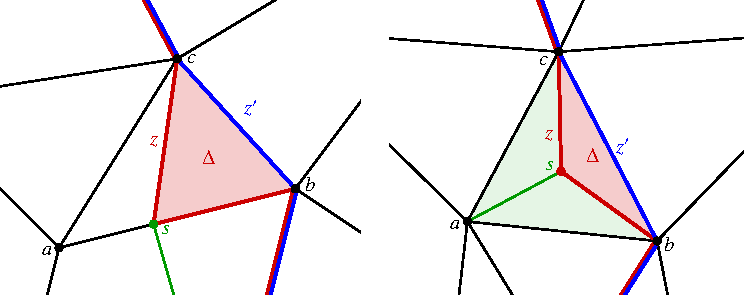
\includegraphics{chapters/120-topologie/images/unterzyklen.pdf}
\caption{Unterteilung eines simplizialen Komplexes mit einem neuen Punkt $s$
auf einer Kante (links) bzw.~im Inneren (rechts) eines 2-Simplex.
Ein Zyklus $z$, der die neue Kante $cs$ verwendet, verwendet auch eine der
neuen Kanten $as$ oder $sb$ ($sb$ im gezeichneten Fall).
Subtraktion des Randes von $\Delta$ verwandelt $z$ in $z-\partial\Delta = z'$.
$z$ und $z'$ sind daher homolog, der Zyklus $z$ ist keine neue
Homologieklasse.
\label{buch:topologie:simplex:fig:unterzyklen}}
\end{figure}
%
Wir müssen zeigen, dass das Hinzufügen eines Unterteilungspunktes 
die einzelnen Vektorräume nicht ändert.
Wir werden keinen vollständigen formellen Beweis geben, sondern
nur anhand einiger Fälle illustrieren, dass die durch den eingefügten
Punkt entstandenen neuen Zyklen homolog sind zu bereits vorhandenen.

Die Unterteilung einer Kante $a_0a_1$ mit einem neuen Punkt $b$ erzeugt
zwei neue Kanten $a_0b$ und $ba_1$.
Da $b-a_0=\partial (a_0b)$ ein Rand ist, sind die Vektoren $a_0\in H_0$
und $b\in H_0$ homolog.
Insbesondere hat sich $H_0$ durch den neuen Punkt nicht verändert.

Ein Unterteilungspunkt $s$ auf einer Kante eines Dreiecks $abc$ fügt auch
eine neu Kante ein, die den neuen Punkt mit dem gegenüberliegenden
Punkt des Dreiecks verbindet.
Die beiden Hälften des Dreiecks haben als Rand jeweils einen Zyklus,
der die neue Kante enthält.

Nehmen wir an, dass diese neue Kante Teil eines Zyklus $z$ ist
(in Abbildung~\ref{buch:topologie:simplex:fig:unterzyklen} links
die Kante $cs$).
Dann muss der Zyklus auch eine der halben Kanten enthalten (den
Teil $sb$ in der Abbildung).
Indem wir den Rand des Dreiecks $\Delta$ subtrahieren, welches die gleiche
halbe Kante enthält, verschwindet sowohl die neue Kante wie auch die
halbe Kante aus dem Zyklus $z$, $z'=z-\partial\Delta$.
Indem wir diese Operation wenn nötig mehrmals durchführen, erhalten
wir einen homologen Zyklus, der im nicht unterteilten Zellenkomplex
liegt.
Das Hinzufügen eines Unterteilungspunktes hat also nur neue Zyklen
hinzugefügt, die homolog sind zu bereits bekannten.

Wir unterteilen jetzt das Dreieck $abc$ mit dem inneren Punkt $s$
(Abbildung~\ref{buch:topologie:simplex:fig:unterzyklen} rechts).
Es entstehen drei neue Dreiecke $abs$, $bcs$ und $cas$ und drei neue
Kanten $as$, $bs$ und $cs$ (in der Abbildung {\color{darkgreen}grün}
eingezeichnet).
Wenn ein Zyklus ${\color{darkred}z}$ im unterteilten $Z_1$ eine der
neuen Kanten enthält, dann muss er auch noch eine weitere solche
Kanten enthalten (die Kanten $cs$ und $bs$ in der Abbildung).
Die beiden Kanten gehören zu genau einem der neuen Dreiecke ($\Delta$
in der Abbildung).
Indem man den Rand dieses Dreiecks vom Zyklus $z$ subtrahiert, erhält
man einen homologen Zyklus $z'=z-\partial\Delta$, der die neuen Kanten
nicht mehr braucht.

Als letztes Beispiel unterteilen wir ein Tetraeder $abcd$ mit
einem inneren Punkt $p$ (Abbildung~\ref{buch:topologie:simplex:fig:zyklus}).
%
% fig-zyklus.tex
%
% (c) 2025 Prof Dr Andreas Müller
%
\begin{figure}
\centering
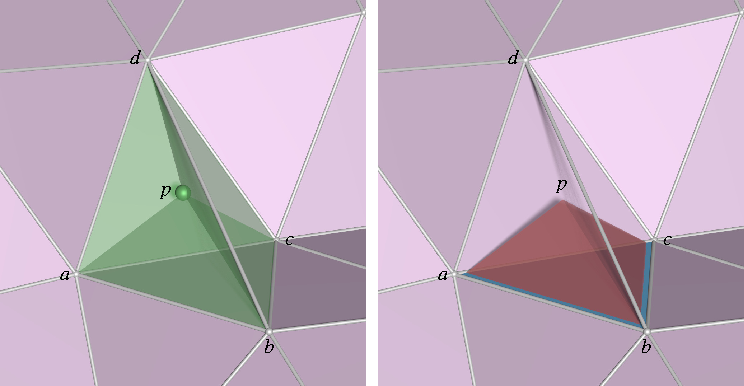
\includegraphics{chapters/120-topologie/images/zyklus.pdf}
\caption{Unterteilung des 3-Simplex $abcd$ mit dem inneren Punkt $p$
(links).
Es entstehen sechs neue 2-Simplizes ({\color{darkgreen}grün}) und vier
neue 3-Simplizes, die durch jeweils drei neue und ein ursprüngliches
2-Simplex berandet sind.
Wenn ein Zyklus (die hellrot dargestellten 2-Simplizes der ``Rückwand'')
eines der neuen 2-Simplizes enthält, dann enthält
er auch noch zwei andere, die eines der vier 3-Simplizes beranden
(rechts, rotes 3-Simplex).
Durch subtrahieren des Randes dieses 3-Simplex bleibt nur
wird der Zyklus auf einen homologen Zyklus mit dem blauen 2-Simplex
reduziert.
\label{buch:topologie:simplex:fig:zyklus}}
\end{figure}
%
Dabei entstehen zu jeder Seitenfläche des Tetraeders ein neues 
Tetraeder und insgesamt sechs neue 2-Simplizes (in der Abbildung
grün dargestellt).
Je zwei der Tetraeder haben jeweils ein neues Dreieck als Seitenfläche
gemeinsam, und je drei eine neue Kante.
Wenn ein Zyklus $z\in Z_2$ eines der neuen Dreieck enthält, dann
muss er auch zwei weitere der neuen Dreiecke enthalten.
Diese drei Dreiecke bestimmen genau eines der neuen Tetraeder.
Subtrahiert man diese Tetraeder von $z$, erhält man einen neuen
Zyklus, der $p$ nicht mehr enthält.
Jeder Zyklus im verfeinerten Zellenkomplex ist also homolog
zu einem Zyklus im ursprünglichen Komplex.
\end{proof}

Der Satz bedeutet, dass die Homologievektorräume mit Hilfe einer
beliebigen Triangulation berechnet werden können.

\begin{beispiel}
\label{buch:topologie:euler:beispiel:tetraeder}
Ein (hohles) Tetraeder $T$ hat vier Ecken, sechs Kanten und vier Seitenflächen.
Das es zusammenhängend ist, wissen wir bereits, dass
$H_0(T,\mathbb{R})=\mathbb{R}$ ist.

Ein eindimensionaler Zyklus ist ein geschlossener Weg.
Enthält ein solcher Weg zwei aneinanderstossende Kanten, dann kann
man den Rand des zugehörige Dreiecks subtrahieren und erhält
einen homologen Zyklus mit einer Kante weniger.
Wiederholung des Prozesses zeigt, dass jeder Zyklus zu 0 homolog
ist, es folgt $H_1(T,\mathbb{R})=0$.

Da das Tetraeder keine dreidimensionalen Simplizes enthält, ist 
$B_2(T)=0$ und folglich $H_2(T,\mathbb{R})=Z_2(T)$.
\end{beispiel}

\begin{beispiel}
\label{buch:topologie:euler:beispiel:kugel}
Da eine Kugel durch Zentralprojektion von einem Tetrader mit
Mittelpunkt im Kugelmittelpunkt trianguliert werden kann, gilt
\[
H_0(S^2,\mathbb{R}) = \mathbb{R},\qquad
H_1(S^2,\mathbb{R}) = 0,\qquad
H_2(S^2,\mathbb{R}) = \mathbb{R}.
\qedhere
\]
\end{beispiel}

%
% fig-torushomologie.tex
%
% (c) 2025 Prof Dr Andreas Müller
%
\begin{figure}
\centering
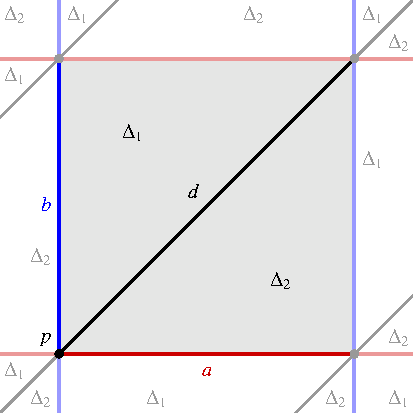
\includegraphics{chapters/120-topologie/images/torushomologie.pdf}
\caption{Triangulation eines Torus mit genau einer Ecke $p$, drei
Kanten $a$, $b$ und $d$ und zwei Dreiecken $\Delta_1$ und $\Delta_2$.
\index{Torus}%
\index{Triangulation}%
Die Kanten gleicher Farbe sind jeweils miteinander zu identifizieren,
sie entsprechen den Kurven gleicher Farbe in
\index{Kurve}%
Abbildung~\ref{buch:topologie:intro:fig:torus}.
\label{buch:topologie:euler:fig:torushomologie}}
\end{figure}
%

\begin{beispiel}
\label{buch:topologie:euler:beispiel:torus}
Zur Berechnung der Homologievektorräume eines zweidimensionalen
Torus $T^2$ lassen sich mit der Triangulation von
Abbildung~\ref{buch:topologie:euler:fig:torushomologie} bestimmen.
Sie enthält genau eine Ecke $p$, drei Kanten $a$, $b$ und $d$ und
zwei Dreiecke $\Delta_1$ und $\Delta_2$.
Die gleichfarbigen Kanten sind jeweils miteinander zu identifizieren.
Sie entsprechen den farbigen Kurven auf dem Torus von
Abbildung~\ref{buch:topologie:intro:fig:torus}.

Da der Torus zusammenhängend ist, ist $H_0(T^2,\mathbb{R})=\mathbb{R}$.

Zwei eindimensionale Zyklen sind leicht zu identifizieren: die 
horizontalen und vertikalen Kanten.
Die diagonale Kante ist homolog zur Verkettung der anderen beiden,
so dass $H_1(T^2,\mathbb{R})$ ein zweidimensionaler Vektorraum
mit den beiden farbigen Kanten als Basis ist.
Somit ist $H_2(T^2,\mathbb{R})=\mathbb{R}^2$.

Da $T^2$ keine dreidimensionalen Simplizes enthält, ist $B_2(T^2)=0$
und folglich $H_2(T^2,\mathbb{R}) = Z_2(T^2)$.
Ein zweidimensionaler Zyklus, der das eine Dreieck enthält, muss auch
das andere enthalten, damit sich die Ränder in der Summe wegheben.
Somit ist $\Delta_1 + \Delta_2$ der einzige Zyklus und es folgt
$H_2(T^2,\mathbb{R})=\mathbb{R}$.
\end{beispiel}

%
% Betti-Zahlen und Euler-Charakteristik
%
\subsection{Betti-Zahlen und Euler-Charakteristik
\label{buch:topologie:simplex:subsection:betti-euler}}
Die Homologievektorräume codieren Information über einen Zellenkomplex,
die wie die Euler-Charakteristik nicht von einer Verfeinerung
abhängt.
Es ist daher nicht unverschämt zu erwarten, dass sich die Euler-Charakteristik
aus den Homologievektorräumen bestimmen lässt.
Dies soll in diesem Abschnitt gezeigt werden.

%
% Betti-Zahlen
%
\subsubsection{Betti-Zahlen}
Die Homologievektorräume sind endlichdimensionale Vektorräume.
Ihre Dimension sagt etwas über die Komplexität des Zellenkomplexes
aus und verdient daher einen eigenen Namen.

\begin{definition}[Betti-Zahlen]
\index{Betti-Zahl}
Die $k$-te \emph{Betti-Zahl} $\beta_k$ ist die Dimension
\[
\beta_k
=
\dim H_k(S,\mathbb{R}).
\]
\end{definition}

\begin{satz}
Eine Unterteilung des Zellenkomplexes ändert die Betti-Zahlen nicht.
\end{satz}

\begin{proof}
Gemäss Satz~\ref{buch:topologie:eulercharakteristik:satz:homologieunterteilung}
ändert die Unterteilung die Homologie-Vektorräume nicht, also ändert sich
auch deren Dimension nicht.
\end{proof}

\begin{beispiel}
\label{buch:topologie:euler:beispiel:betti-tetraeder}
Im Beispiel~\ref{buch:topologie:euler:beispiel:tetraeder} wurden die 
Homologievektorräume eines Tetraeders und anschliessend in
Beispiel~\ref{buch:topologie:euler:beispiel:kugel} einer Kugel berechnet.
Daraus lassen sich die Bettizahlen
\[
\beta_0(T) = \beta_0(S^2) = 1,\qquad
\beta_1(T) = \beta_1(S^2) = 0,\qquad
\beta_2(T) = \beta_2(S^2) = 1
\]
ablesen.
\end{beispiel}

\begin{beispiel}
\label{buch:topologie:euler:beispiel:betti-torus}
Im Beispiel~\ref{buch:topologie:euler:beispiel:torus} wurden die 
Homologievektorräume eines Torus $T^2$ berechnet.
Daraus lassen sich die Bettizahlen
\[
\beta_0(T^2) = 1,\qquad
\beta_1(T^2) = 2,\qquad
\beta_2(T^2) = 1
\]
ablesen.
\end{beispiel}

%
% Euler-Charakteristik
%
\subsubsection{Euler-Charakteristik}
Die alternierende Summe der Betti-Zahlen aus den
Beispielen~\ref{buch:topologie:euler:beispiel:betti-tetraeder}
und \ref{buch:topologie:euler:beispiel:betti-torus} ergibt
\begin{align*}
1-0+1 &= 2 \\
1-2+1 &= 0.
\end{align*}
Dies stimmt mit den in
Tabelle~\ref{buch:topologie:intro:table:eulercharakteristik}
protokollierten Euler-Charakteristiken überein.
Dies suggeriert, dass sich die Euler-Charakteristik bereits aus
den Betti-Zahlen bestimmen lässt.
Der folgende Satz zeigt, dass dies tatsächlich möglich ist.

\begin{satz}
\label{buch:topologie:simplex:satz:euler-betti}
Die Euler-Charakteristik ist durch die Betti-Zahlen bestimmt,
es gilt
\[
\chi(S)
=
\sum_{k=0}^n (-1)^k \beta_k.
\]
\end{satz}

\begin{proof}
Die Eulercharakteristik ist als alternierende Summe der Anzahl der Simplizes 
jeder Dimension definiert.
Die Anzahl tritt als Dimension der Vektorräume $C_k$ auf.
$\dim C_0$ ist die Anzahl der Ecken, $\dim C_1$ die Anzahl der Kanten,
$\dim C_2$ die Anzahl der Dreieck usw.
Die Euler-Charakteristik kann man daher auch schreiben als
\[
\chi(S)
=
\sum_{k=0}^n (-1)^k \dim C_k.
\]
Um die Notation zu vereinfachen, schreiben wir für die alternierende
Summe der Betti-Zahlen als
\[
\chi_H(S)
=
\sum_{k=0}^n
(-1)^k \beta_k
=
\sum_{k=0}^n
(-1)^k \dim H_k(S,\mathbb{R}),
\]
wobei die Notation andeuten soll, dass dies die ``homologisch''
definierte Euler-Cha\-rak\-te\-ris\-tik ist.

Die Homologievektorräume sind ebenfalls endlichdimensionale Vektorräume.
Ihre Dimension ergibt sich aus
\[
\dim H_k(S)
=
\dim Z_k(S) - \dim B_k(S).
\]
Die Dimensionen von $Z_k$ und $B_k$ sind aber mit den Dimensionen von
$C_k$ über den Randoperator verbunden.

Die Ränder $B_k$ sind der Bildraum des Operators $\partial_{k+1}$, seine
Dimension wird durch den Rang gegeben:
\begin{equation}
\dim B_k
= 
\operatorname{Rang} \partial_{k+1}.
\label{buch:topologie:simplex:eqn:dimb}
\end{equation}

Die Zyklen $Z_k$ bilden den Kern des Operators $\partial_k$, so dass
die Dimension von $Z_k$
\begin{equation}
\dim Z_k
=
\dim\ker \partial_k
=
\dim C_k - \operatorname{rank} \partial_k
\label{buch:topologie:simplex:eqn:dimz}
\end{equation}
ist.

Aus den Gleichungen folgt jetzt für die Betti-Zahlen
\begin{equation}
\dim H_k(S,\mathbb{R})
=
\dim Z_k - \dim B_k
=
\dim C_k - \operatorname{rank} \partial_k
- \operatorname{rank}\partial_{k+1}.
\label{buch:topologie:simplex:eqn:dimh}
\end{equation}
Daraus kann man jetzt die alternierende Summe der Betti-Zahlen
ausrechnen
\begin{align*}
\chi_H(S)
&=
\sum_{k=0}^n (-1)^k \dim H_k(S,\mathbb{R})
\\
&=
\sum_{k=0}^n (-1)^k\bigl(
\dim C_k - \operatorname{rank} \partial_k
- \operatorname{rank}\partial_{k+1}
\bigr)
\\
&=
\sum_{k=0}^n (-1)^k\dim C_k
-\sum_{k=0}^n(-1)^k\operatorname{rank}\partial_k
-\sum_{k=1}^n(-1)^k\operatorname{rank}\partial_{k+1}.
\intertext{Die erste Summe ist die Euler-Charakteristik.
In der letzten Summe verschieben wir den Summationsindex um 1 und
erhalten die leichter zu vergleichenden Summen}
&=
\chi(S)
-\sum_{k=0}^n(-1)^k\operatorname{rank}\partial_k
+\sum_{k=1}^{n+1}(-1)^{k}\operatorname{rank}\partial_{k}.
\intertext{Bis auf den ersten Term der linken Summe und den letzten Term
der rechten Summe haben sich die Terme der beiden Summen gegenseit weg,
so dass nur}
&=
\chi(S)
-\operatorname{rank}\partial_0
+(-1)^{n+1}\operatorname{rank}\partial_{k+1}
\end{align*}
übrig bleibt.
Der Operator $\partial_0$ ist aber der Nulloperator und hat daher Rang 0.
Da $S$ ein $n$-dimensionaler Zellenkomplex ist, gibt es keine
$(n+1)$-Zyklen.
Somit ist auch $\partial_{n+1}=0$ und $\operatorname{rank}\partial_{n+1}=0$
und damit $\chi_H(S) = \chi(S)$.
\end{proof}

Es ist daher durchaus gerechtfertigt, einem Kettenkomplex $C=(C_*,\partial_*)$
eine Euler-Charakteristik 
\[
\chi(C)
=
\chi(C_*,\partial_*)
=
\sum_{k\in\mathbb{N}} (-1)^k\dim H_k(C)
\]
zuzuordnen.
\index{Euler-Charakteristik!eines Kettenkomplexes}%
Der Satz~\ref{buch:topologie:simplex:satz:euler-betti}
zeigt dann, dass die früher definierte Euler-Charakteristik des
Zellenkomplexes dasselbe ist wie die Euler-Charakteristik des
zugehörigen Kettenkomplexes.
Der eben gelieferte Beweis des
Satz~\ref{buch:topologie:simplex:satz:euler-betti}
zeigt ausserdem, dass diese Euler-Charakteristik eines beliebigen
Kettenkomplexes, unabhängig davon, ob er als Kettenkomplex eines
Zellenkomplexes gefunden wurde, ebenfalls als alternierende Summe
\[
\chi(C)
=
\sum_{k\in\mathbb{N}} (-1)^k \dim C_k
\]
berechnet werden kann, wenigstens wenn die Vektorräume $C_k$ alle
endlichdimensional sind.





%
% Morse-Theorie
%
\section{Morse-Theorie
\label{buch:topologie:section:morse}}
\kopfrechts{Morse-Theorie}
Die Morse-Theorie stellt einen Zusammenang zwischen der Topologie einer 
Mannigfaltigkeit und den kritischen Punkten einer Funktion auf der
Mannigfaltigkeit.
Die grossräumigen Eigenschaften einer Mannigfaltigkeit sind also
in den Eigenschaften von Funktionen in einigen wenigen, isolierten
Punkten einer Funktion codiert.

%
% Zerlegung einer zweidimensionalen Mannigfaltigkeit
%
\subsection{Zerlegung einer zweidimensionalen Mannigfaltigkeit}
%
% fig-karte.tex
%
% (c) 2025 Prof Dr Andreas Müller
%
\begin{figure}
\centering
\includegraphics[width=\textwidth]{chapters/120-topologie/images/karte.png}
\caption{Die Hähenlinien sind die Niveaulinien der auf der Erdoberfläche
definierten Funktion, die die Höhe eines Punktes angibt.
Die Niveaulinien zerlegen die Oberfläche der Erde in Streifen oder Ringe.
Die Idee der Morse-Theorie ist, dass sich die Topologie der Erdoberfläche
aus diesen Elementen rekonstruieren lässt.
\label{buch:topologie:morse:fig:karte}}
\end{figure}
%
%
% fig-relief.tex
%
% (c) 2025 Prof Dr Andreas Müller
%
\begin{figure}
\centering
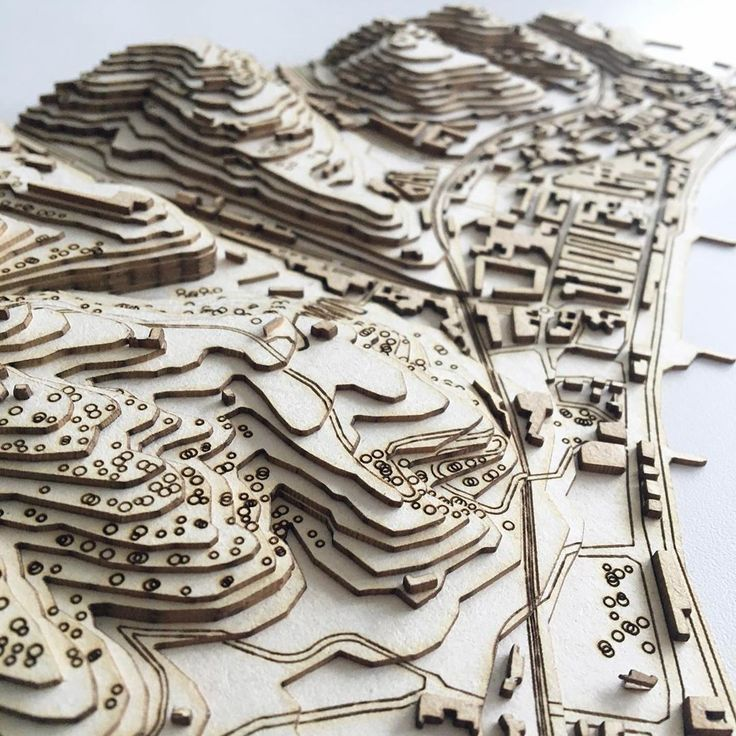
\includegraphics[width=0.7\textwidth]{chapters/120-topologie/images/relief.jpg}
\caption{Rekonstruktion einer Approximation der Topographie aus den
\index{Topographie}%
Höhenlinien mit Hilfe von Platten, die entlang der Höhenlinien ausgeschnitten
worden sind.
\label{buch:topologie:morse:fig:relief}}
\end{figure}
%
Aus einer glatten Funktion $f\colon M\to\mathbb{R}$ lässt
sich eine natürliche Zerlegung einer Mannigfaltigkeit konstruieren.
In Abbildung~\ref{buch:topologie:morse:fig:karte} zeigt eine 
topographische Karte.
Die Höhenlinien sind die Niveaulinien der Funktion, die einem
Punkt seine Höhe über dem Meeresspiegel zuordnet.
Die Höhenlinien zerlegen die Karte in Streifen, Ringe und andere
zweidimensionale Gebiete.
Der geübte Kartenleser ist in der Lage, aus den Höhenlinien eine
Vorstellung der Topographie zu rekonstruieren.
Man kann aber auch aus den Höhenlinien ein massstäbliches Modell
des Geländes bauen.
Für jedes Niveau schneidet man das von der Höhenlinie berandete Gebiet
aus einer Holzplatte aus und schichtet die erhaltenen Platten
wie in Abbildung~\ref{buch:topologie:morse:fig:relief} gezeigt
auf.
Es entsteht eine Approximation des Geländes.

Wir betrachten jetzt eine einzelne Höhenlinie.
Die Höhenlinie zur Höhe $c$ ist die Menge der Punkte
\[
H_c
=
\{ p\in M\mid f(p) = c \}.
\]
Wenn wir $c$ um einen kleinen Betrag $\Delta c$ verschiebt sich
die Höhenlinie in eine Richtung senkrecht auf die Höhenlinie.
Ein positives $\Delta c$ bedeutet, dass wir eine Höhenlinie weiter
oben am Berg suchen.
Ist $\Delta c$ klein genug, ist die neue Höhenlinie $H_{c+\Delta c}$
meistens eine Kurve, die in unmittelbarer Nähe der Kurve $H_c$.
die Veränderung von $c$ hat also keine wesentlichen Auswirkungen
auf die Gestalt der Höhenlinie, wenigstens wenn die Höhenlinie
immer an einem Hang entlang verläuft.

Die Voraussetzung, dass die Höhenlinie dem Hang entlang verlaufen
muss, damit eine kleine Höhenänderung keine Auswirkung auf die
Gestalt der Kurve hat, ist zum Beispiel bei einem Gipfel verletzt.
Sei $p$ ein lokales Maximum der Funktion $f$ und U eine so kleine
Umgebung von $p$, dass die Höhenlinie $H_c = \{p\}$ nur den Punkt $p$
enthält.
Vergrössert man $c$ um $\Delta c>0$, verschwindet der Punkt $p$,
die Höhenlinie $H_{c+\Delta c}=\emptyset$ ist leer.
Bei einer Verkleinerung wird wird die Höhenline $H_{c+\Delta c}$ zu
einer geschlossenen Kurve, die den Punkt $p$ umschliesst
(Abbildung~\ref{buch:topologie:morse:fig:karte}, Umgebung des Punktes 1384),
wenigstens wenn die zweiten Ableitungen von $f$ an der Stelle $p$
nicht verschwinden.

Ein ganz anderes Bild bietet sich bei einem Pass der Höhe $c$.
Auch ein Sattelpunkt der Fläche ist eine Stelle, an der
alle partiellen ersten Ableitungen verschwinden.
Die Menge $H_c$ besteht aber nicht aus einem Punkt, vielmehr
kommen im Punkt $p$ vier Höhenlinien zusammen.
Für grössere und kleiner Werte verschwindet der Schnittpunkt,
es bleiben zwei nicht verbundene Höhenlinie wie in
bei links unterhalb der Büelhöchi in
Abbildung~\ref{buch:topologie:morse:fig:karte}.

Diese Diskussion zeigt, dass wesentliche Eigenschaften der Topographie
aus Punkten abzulesen sind, an denen die ersten Ableitungen verschwinden,
die zweiten Ableitungen aber nicht (was das genau heisst, muss noch
definiert werden).

%
% Index einer Nullstelle
%
\subsection{Kritische Punkte und ihr Index}
In diesem Abschnitt ist $M$ eine $n$-dimensionale Mannigfaltigkeit.
Wir betrachten die Menge $C^\infty(M)$ der beliebig oft stetig
differenzierbare Funktionen auf $M$.

%
% Kritische Punkte
%
\subsubsection{Kritische Punkte}
%
% fig-morse.tex
%
% (c) 2025 Prof Dr Andreas Müller
%
\begin{figure}
\centering
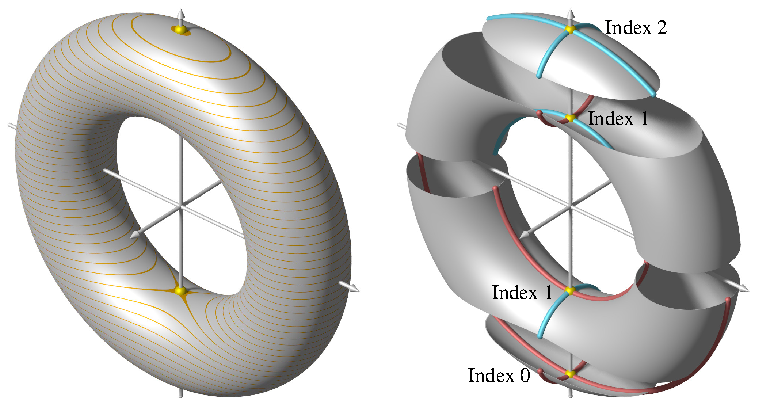
\includegraphics{chapters/120-topologie/images/morse.pdf}
\caption{Links: Torus mit Höhenlinien der Funktion $f(p) = z(p)$ für Punkte
$p$ auf dem Torus.
\index{Torus}%
Kritische Punkte von $f$ sind gelb eingezeichnet.
\index{kritischer Punkt}%
Rechts: Der Torus lässt sich in Teile zerlegen, die jeweils genau
einen kritischen Punkte enthalten. Aus den Indizes der kritischen Punkte
\index{Index}%
lassen sich topologische Eigenschaften der Mannigfaltigkeit rekonstruieren.
\label{buch:topologie:fig:morse}}
\end{figure}
%
Die äussere Ableitung einer Funktion $f\colon M\to\mathbb{R}$ 
wird ein einer Karte $\varphi_\alpha\colon U_\alpha\to\mathbb{R}^n$
zu einer Funktion der $n$ Koordinaten, die wir $f(x^1,\dots,x^n)$
schreiben.
Bei einem Maximum oder Minimum der Funktion verschwinden alle ersten
Ableitungen, in dieser Karte wird die äussere Ableitung
\[
df
=
\frac{\partial f}{\partial x^1}\,dx^1
+
\dots
+
\frac{\partial f}{\partial x^n}\,dx^n
=
0.
\]
Wechselt man das Koordinatensystem, ändert dies an der Tatsache, dass
$df=0$ ist, nichts.

\begin{definition}[kritischer Punkt]
\index{kritischer Punkt}%
\index{Punkt!kritisch}%
\index{kritischer Wert}%
\index{Wert!kritisch}%
Ein \emph{kritischer Punkt} einer glatten Funktion $f$ auf einer
differenzierbaren Mannigfaltigkeit ist ein Punkt $p\in M$, bei dem
$df(p)=0$ ist.
Der Wert $c=f(p)$ in einem kritischen Punkt $p$ heisst
\emph{kritischer Wert} der Funktion f.
\end{definition}

%
% Die hessesche Matrix
%
\subsubsection{Die hessesche Matrix}
Sei $p$ ein kritischer Punkt der Funktion $f$ auf der Mannigfaltigkeit $M$
mit dem kritischen Wert $c=f(p)$.
In einem Koordinatensystem in der Umgebung des Punktes $p$ kann die Funktion
durch die Taylor-Reihe 
\begin{align}
f(x^1,\dots,x^n)
&=
f(p)
+
\sum_{k=1}^n \frac{\partial f}{\partial x^k}(p) (x^k-x^k(p))
\\
&\qquad\mathstrut
+
\sum_{k,l=1}^n
\frac{\partial^2 f}{\partial x^k\,\partial x^l}(p)
(x^k-x^k(p))(x^l-x^l(p))
+
o(|x-p|^2)
\notag
\\
&=
c
+
\sum_{k,l=1}^n
\frac{\partial^2 f}{\partial x^k\,\partial x^l}(p)
(x^k-x^k(p))(x^l-x^l(p))
+
o(|x-p|^2)
\label{buch:topologie:morse:eqn:quadratisch}
\end{align}
approximiert werden.
Die Matrix der zweiten Ableitungen heisst auch die \emph{hessesche Matrix}
$H$ an der Stelle $p$ mit den Einträgen
\[
h_{ik}
=
\frac{\partial^2 f}{\partial x^i\,\partial x^k}(p).
\]

In einer Dimension besteht die hessesche Matrix nur aus der zweiten
Ableitung $f''(p)$ der Funktion.
Wenn Sie nicht verschwindet lässt sich daraus ableiten, ob der
kritische Punkt ein lokales Maximum oder Minimum ist.
In höheren Dimensionen ist die Situation etwas komplizierter

%
% Nichtentartete quadratische Formen
%
\subsubsection{Nichtentartete quadratische Formen}
Wir möchten sicherstellen, dass wir zuverlässige Aussagen über die
Form der \emph{Niveaumengen} $H_c=\{p\in M\mid f(p)=c\}$ in der
Umgebung eines kritischen Punktes machen können.
Dazu muss der quadratische Term in
\eqref{buch:topologie:morse:eqn:quadratisch}
immer gegenüber den Termen höherer Ordnung dominieren.
Dies ist nur möglich, wenn der quadratische Ausdruck
\[
H(v)
=
\sum_{k,l=1}^n
\frac{\partial^2 f}{\partial x^k\,\partial x^l}
v^k v^l
\]
nicht entartet im Sinne der folgenden zwei Definitionen ist.

\begin{definition}[quadratische Form]
Ist $H$ eine symmetrische Matrix, dann ist schreiben wir
\[
H(v)
=
v^tHv
=
\sum_{i,k=1}^n = h_{ik} v^iv^k
\]
und sagen, dass $H(v)$ eine \emph{quadratische Form} ist.
\index{quadratische Form}%
\end{definition}

Die \emph{Polarisationsformel} \cite[p.~347]{buch:linalg} ermöglicht,
aus der quadratischen Form
\index{Polarisierungsformel}
$H(v)$ die Bilinearform
\[
\langle u,v\rangle_H
=
u^tHv
\]
zu rekonstruieren.
Die Formel lautet
\[
\langle u,v\rangle_H
=
\frac14\bigl(H(u+v) - H(u-v)\bigr).
\]
Damit können jetzt auch die Matrixelemente
$h_{ik} = \langle\vec{e}_i,\vec{e}_k\rangle_H$ von $H$
wiedergewinnen.
Man verliert also nichts, wenn man nur die quadratische Form kennt,
wie sie in der Taylor-Reihe auftritt.

\begin{definition}[entartete quadratische Form]
\label{buch:topologie:morse:def:entartet}
Eine quadratische Form mit Matrix $H$ heisst \emph{entartet}, wenn
die Matrix $H$ singulär ist.
\index{entartet}%
\end{definition}

Die Bedingung der Definition~\ref{buch:topologie:morse:def:entartet}
bedeutet, dass es einen Vektor $v$ mit $Hv=0$ gibt.
Für einen solchen Vektor gilt $\langle u,v\rangle_H=0$
für alle Vektoren $u$.
Die Bedingung verhindert nicht, dass es Vektoren gibt, für die
$H(u)=0$.
Die quadratische Form mit der Matrix
\[
H=
\begin{pmatrix}
1&0\\0&-1
\end{pmatrix}
\]
ist sicher nicht entartet, aber wegen
\[
v^tHv
=
(v^1)^2-(v^2)^2
\]
gilt
\[
v=\begin{pmatrix}1\\1\end{pmatrix}
\qquad\Rightarrow\qquad
H(v) = 0.
\]
Es gibt also eine Richtung, für die die quadratische Form verschwindet.
Für die Standardbasisvektoren gilt allerdings
$ H(e_1)=1$ und $H(e_2)=-1$.
Die Funktion $z=H(v^1,v^2)$ kann als Sattelfläche dargestellt werden.
Auf einer Sattelfläche gibt es Richtungen, in denen sich $H$ nicht
verändert und Richtungen, für die $H$ zu- bzw.~abnimmt.

Die Bedingung, dass die hessesche Matrix $H$ nicht entartet sein darf,
entspricht der Bedingung für Funktionen einer Variablen, dass die zweite
Ableitung nicht verschwinden darf.
Sie stellt sicher, dass der quadratische Term in der Nähe des kritischen
Punktes in alle Richtungen das Vorhalten der Funktion dominiert.

%
% Der Index eines kritischen Punktes
%
\subsubsection{Der Index eines kritischen Punktes}
Die hessesche Matrix $H$ mit den Einträgen
\[
h_{kl} = \frac{\partial^2 f}{\partial x^k\,\partial x^l}
\]
ist in einem nicht entarteten kritischen Punkt eine symmetrische
Matrix.
Da symmetrische Matrizen durch orthogonale Transformationen
diagonalisierbar sind, können wir das Koorinatensystem mit
einer orthogonalen Matrix so drehen, dass $H$ die Form
\[
H(v)
=
\sum_{i=1}^n \lambda_i (v^i)^2
\]
bekommt.
Die $\lambda_i$ sind die Eigenwerte der Matrix $H$, keiner
der Eigenwerte verschwindet.
Durch Streckung der Koordinatenachse $x^1$ mit dem Faktor
$\!\sqrt{|\lambda_i|}$  mittels
$y^i = \!\sqrt{|\lambda_i|}x^i$ kann die Entwicklung
\eqref{buch:topologie:morse:eqn:quadratisch}
in die Form
\begin{align*}
f(y^1,\dots,y^n)
&=
c
+
\operatorname{sgn}(\lambda_1)\,(y^1)^2
+
\dots
+
\operatorname{sgn}(\lambda_n)\,(y^n)^2
\end{align*}
gebracht werden.

Es kommt also nur auf die Vorzeichen der Eigenwerte an.
Bei einem Koordinatenwechsel ändert sich die Matrix $H$ der zweiten
Ableitungen, aber die Anzahl der positiven und negativen Eigenwerte
bleibt erhalten.

\begin{definition}[Index]
\index{Index einer quadratischen Form}%
Der \emph{Index} einer nicht entarteten quadratischen Form $H$ ist die
Anzahl $k$ der negativen Eigenwerte.
Der Index wird mit $\operatorname{Ind}H$ bezeichnet.
\index{Index einer quadratischeN Form}%
\index{Ind@$\operatorname{Ind}$}%
\end{definition}

Der Index ist eine Grösse, die auf kleine Störungen der Funktion
unempfindlich ist, solange der Punkt ein kritischer Punkt bleibt.

%
% Morse-Funktionen
%
\subsubsection{Morse-Funktionen}
Wir betrachten die Funktion
\[
f_t(x)
=
x^3-tx
=
(x-\!\sqrt{t})x(x+\!\sqrt{t})
\]
mit dem Parameter $t$, wobei die Faktorisierung nur für $t\ge 0$ möglich
ist.
Die Ableitungen sind
\begin{align*}
f'_t(x)
&=
3x^2-t
=
(\!\sqrt{3}x-\!\sqrt{t})
(\!\sqrt{3}x+\!\sqrt{t})
\\
f''_t(x)
&=
6x.
\end{align*}
Für $t> 0$ hat die Funktion zwei kritische Punkte bei $\pm\!\sqrt{t/3}$,
die nicht entartet sind, weil die zweite Ableitung $\ne 0$ ist.
Die beiden kritischen Punkte haben verschiedenen
Index $0$ für $t=\!\sqrt{t/3}$
und $1$ für $t=-\!\sqrt{t/3}$.
Für $t<0$ gibt es keine kritischen Punkte.
Für $t=0$ gibt es den kritischen Punkt $x=0$, der aber entartet ist.
Die Differenz der Anzahl positiver und negativer zweiter Ableitungen
bei den kritischen Punkten bleibt bei der Deformation der Funktion 
mithilfe des Paramters $t$ gleich.
Dies suggeriert, dass die Betrachtung der kritischen Punkte etwas
über die topologischen Eigenschaften aussagt.
Dies funktioniert aber nicht für den Fall $t=0$, weil der kritische
Punkt dort entartet ist.
Für die topologische Untersuchung sind daher nur Funktionen geeignet,
die keine entarteten kritischen Punkte haben.

\begin{definition}[Morse-Funktion]
\index{Morse-Funktion}%
Eine {\em Morse-Funktion} auf einer differenzierbaren Mannigfaltigkeit
$M$ ist eine stetig differenzierbare Funktion $f\colon M\to\mathbb{R}$,
deren kritische Punkte alle nicht entartet sind.
Der \emph{Index} $\operatorname{Ind}_pf$ des kritischen Punktes ist der Index
\index{Index eines kritischen Punktes}%
der hesseschen Matrix im Punkt $f$:
\[
\operatorname{Ind}_pf
=
\operatorname{Ind}\biggl(
\frac{\partial^2 f}{\partial x^i\,\partial x^k}(p)
\biggr).
\]
\index{Ind_pf@$\operatorname{Ind}_pf$}%
\end{definition}

Nach obiger Diskussion ist das Einführungsbeispiel $f_t(x)$ also für
$t\ne0$ eine Morse-Funktion auf $\mathbb{R}$.

Für Flächen $M$, die durch Einbettung in den dreidimensionalen Raum
$\mathbb{R}^3$ gegeben sind, sind die Koordinatenfunktion
$x(P)$, $y(P)$ und $z(P)$ natürlich Kandidaten für Morse-Funktionen.
Die Einbettung der Kugel
\[
S^2
=
\{ (x,y,z)\mid x^2+y^2+z^2=1 \}
\subset
\mathbb{R}^3
\]
liefert so drei Morse-Funktionen auf der Kugeloberfläche, die jeweils
genau zwei kritische Punkte mit Indizes 2 für das Maximum und
0 für das Minimum haben.
Man kann sich vorstellen, dass durch Deformation der Kugeln weitere
kritische Punkt der Koordinatenfunktionen entstehen können.
Ein zweites lokales Maximum wird aber immer mit einem Sattelpunkt
verbunden sein, der Index $1$ hat.

%
% Rekonstruktion
%
\subsection{Rekonstruktion}
Aus den Eigenschaften einer Morse-Funktion können viele topologische
Eigenschaften einer differenzierbaren Mannigfaltigkeit rekonstruiert
werden.
Die früher in Abschnitt~\ref{buch:topologie:section:simplex}
mit Hilfe der Homologiegruppen definierte Euler-Charakteristik
lässt sich zum Beispiel bereits mit aus einer Morse-Funktion
ableiten.

%
% Kugeln
%
\subsubsection{Kugeln}
Der folgende Satz zeigt, dass die Eigenschaften einer Morse-Funktion
tatsächlich bereits die topologischen Eigenschaften einer Mannigfaltigkeit
festlegen können.

\begin{satz}
\label{buch:topologie:morse:satz:kugeln}
Sei $M$ eine kompakte, $n$-dimensionale differenzierbare Mannigfaltigkeit
und $f$ eine Morse-Funktion mit genau zwei kritischen Punkten, dann ist
$M$ eine $n$-dimensionale Kugel.
\end{satz}

\begin{proof}[Beweisidee]
%
% fig-kartoffel.tex
%
% (c) 2025 Prof Dr Andreas Müller
%
\begin{figure}
\centering
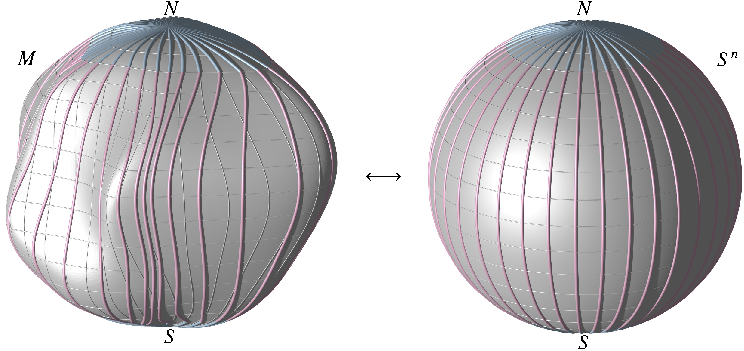
\includegraphics{chapters/120-topologie/images/sphere.pdf}
\caption{Konstruktion von Karten für eine kompakte Mannigfaltigkeit mit
einer Morse-Funktion mit genau zwei kritischen Punkten.
Ausserhalb einer Umgebung des Maximums und des Minimums können die Bahnen
(hellrot)
des Gradienten der Morse-Funktion als Koordinatenlinien (links) verwendet
und auf die Meridiane einer Kugel (rechts) abgebildet werden.
Dies zeigt, dass die Mannigfaltigkeit homömorph zu einer Kugel ist, die
Knicke zwischen den hellblauen Meridianen und den Bahnen zeigen aber auch,
dass die Mannigfaltigkeit nicht diffeomorph zu einer Kugel zu sein brauchtt.
\label{buch:topologie:morse:fig:kartoffel}}
\end{figure}
%
Man muss aus der Funktion $f$ eine bijektive stetige und Abbildung
von $M$ auf eine $n$-dimensionale Kugel konstruieren, deren
Umkehrungabbildung ebenfalls stetig ist.

Da die Mannigfaltigkeit $M$ kompakt ist, nimmt $f$ auf $M$ mindestens
ein Maximum und ein Minimum an.
Diese sind automatisch kritische Punkte.
Weil $f$ eine Morse-Funktion ist, sind sie auch nicht entartet.
Wir bezeichnen den Punkt, in dem $f$ das Maximum annimmt, mit $N$,
und den Punkt, in dem $f$ das Minimum annimt mit $S$
(Abbildung~\ref{buch:topologie:morse:fig:kartoffel} links).
Durch Skalarierung der Funktion $f$ kann man ohne Beschränkung der
Allgemeinheit annehmen, dass $f(N)=1$ und $f(S) = -1$ ist.

Die Funktion $f$ kann als die $n+1$-Koordinate einer Abbildung von $M$ 
auf eine Kugel betrachtet werden.
Für die anderen Koordinatenfunktionen benutzen wir, dass wir annehmen
dürfen, dass es auf $M$ eine riemannsche Metrik gibt.
Mit ihre konstruieren wir das Vektorfeld $X$ des Gradienten der 1-Form $df$.

Da $M$ eine Mannigfaltigkeit ist, gibt es eine Karte um den Punkt $N$,
so dass die Kartenabbildung ein Diffeomorphismus einer Umgebung von $N$
mit einem $n$-dimensionalen Ball ist.
Diese Abbildung kann verwendet werden, um einen Homöomorphismus 
mit der Polkappe der $n$-Dimensionalen Kugeloberfläche in 
Abbildung~\ref{buch:topologie:morse:fig:kartoffel} rechts zu
konstruieren.
Sie wird durch die hellblauen Radien symbolisiert.
Dieselbe Konstruktion kann natürlich auch auf eine Umgebung von $S$
angewendet werden.

Zur Vervollständigung wird jetzt noch eine Abbildung der Umgebung des
Äquators benötigt.
Dazu konstruieren wir für jeden Punkt am Ende eines blauen Radius die
hellrote eingezeichneten Kurven.
Sie sind Lösungskurven des Gradienten der Funktion $f$.
Die Bahnen können sich nicht schneiden und sie hängen stetig vom
Anfangspunkt ab.
Sie liefern daher einen Homöomorphismus mit den hellroten Kurven
auf der Kugeloberfläche.

Zu jedem Anfangspunkt einer hellroten Kurve gibt es den Endpunkt wo
die Kurve in den Rand des $n$-dimensionalen Balles in der Umgebung
von $S$ eintritt.
Dies ist die Kartenwechselabbildung für einen Atlas von $M$.
Er zeigt, dass $M$ und $S^n$ homöomorph sind.
\end{proof}

Der Beweis von Satz~\ref{buch:topologie:morse:satz:kugeln} versucht
nicht, einen Diffeomorphismus zu konstruieren.
Dies äussert sich zum Beispiel in den ``Knicken'' der Meridiankurven
in der Abbildung~\ref{buch:topologie:morse:fig:kartoffel}, die andeuten,
dass die Kartenwechselabbildungen nicht differenzierbar zu sein brauchen.
Diffeomorphie ist auch nicht zu erwarten, denn man kann zeigen, dass es
Mannigfaltigkeiten gibt, die topologisch zwar $n$-dimensionale
Sphären sind, aber nicht diffeomorph sind zur bekannten differenzierbaren
Mannigfaltigkeit $S^n$.

In diesem Zusammenhang ist auch der Satz von Poincaré-Bendixson,
der in Kapitel~\ref{chapter:poinbendix} vorgestellt wird, zu beachten.
Er besagt, dass ein Vektorfeld auf einer Kugeloberfläche $S^2$ nur
ganz bestimmte Lösungskurven haben kann.
Der Gradient einer Morse-Funktion wie in
Satz~\ref{buch:topologie:morse:satz:kugeln}
ist ein Vektorfeld mit nur zwei kritischen Punkten.
Für diesen Fall sagt der Satz von Poincaré-Bendixson, dass die
\index{Poincare-Bendixson@Poincaré-Bendixson}%
Lösungskurven Bahnen sind, die also $\omega$-Limesmengen die 
\index{o-Limesmenge@$\omega$-Limesmenge}%
\index{a-Limesmenge@$\alpha$-Limesmenge}%
\index{Alpha-Limesmenge}%
\index{Omega-Limesmenge}%
Maximumstelle haben, und als $\alpha$-Limesmenge die Minimumstelle.

%
% Homotopietyp und Morse-Funktion
%
\subsubsection{Homotopietyp und Morse-Funktionen}
Eine Morse-Funktion codiert in ihren kritischen Punkten Information
über die Struktur der Mannigfaltigkeit.
Auf einer kompakten Mannigfaltigkeit findet man immer einen kritischen
Punkt mit Index $0$ für die Minimumstelle und einen mit Indes $n$ für
das Maximum.
\index{Sattelpunkt}%
Weitere kritische Punkte treten auf für Sattelpunkte.

Abbildung~\ref{buch:topologie:fig:morse} zeigt einen zweidimensionalen
Torus.
Im ``Loch'' des Torus hat die $z$-Koordinatenfunktion zwei kritische Punkte
mit Index $1$.
Die Abbildung zeigt auch, wie der Torus schrittweise aufgebaut werden
kann.
Man beginnt ganz unten mit einer Kreisscheibe.
Der nächsthöhere kritische Punkt zeigt an, dass zwischen zwei Punkten
des Randes eine ``Brücke'' gebaut werden muss.
Es entsteht jetzt eine Fläche mit zwei kreisförmigen Rändern.
Der nächste kritische Punkt zeigt an, dass die beiden Ränder mit
einer weiteren Brücke verbunden werden müssen.
Damit verschmelzen die beiden Randkreise wieder zu einem.
Schliesslich kann der Randkreis mit einer ``Kappe'' aus einer
zweidimensionalen Kreissscheibe geschlossen und damit eine
Mannigfaltigkeit konstruiert werden, die bis auf Deformation mit dem
Torus übereinstimmt.

Man nennt einen topologischen Raum, der schrittweise aus einem Punkt
durch Anfügen von $k$-dimensionaler Kreisscheiben aufgebaut werden kann,
einen CW-Komplex.
\index{CW-Komplex}%
Ein solcher codiert im Wesentlichen alle Informationen, die man braucht,
um einen topologischen Raum bis auf Deformation zu charakterisieren.

Die kritischen Punkte einer Morse-Funktion bestimmen bereits viele
Aspekte eines CW-Komplexes.
Allerdings ist die Information über die Indizes der kritischen Punkte
nicht unbedingt ausreichend für eine exakte Rekonstruktion der
Mannigfaltigkeit.
Zum Beispiel gibt es auch im Beispiel des Torus die Möglichkeit,
den zweiten kritischen Punkt mit Index $1$ durch eine Brücke zu
realisieren, die zwei Punkte auf dem gleichen Randkreis verbindet.
So würden drei Randkreise entstehen.
Da die Morse-Funktion nur noch einen weiteren kritischen Punkt hat,
könnte nur einer der Randkreise mit einer ``Kappe'' geschlossen
werden.
Im Nachhinein leiten wir daraus ab, dass der Schritt, zwei Punkte des
gleichen Randkreises zu überbrücken, nicht aufgeht.
Es ist allerdings nicht klar, wie eine solche Schlussfolgerung
für eine grosse Zahl von kritischen Punkten möglich sein könnte.

Die Information in den kritischen Punkten einer Morse-Funktion reicht
aber aus, um wenigstens die Betti-Zahlen der Mannigfaltigkeit
wenn nicht zu bestimmen, so doch mindestens einzuschränken.

%
% Euler-Charakteristik
%
\subsubsection{Euler-Charakteristik}
Die Diskussion kritischen Punkte auf dem Torus von
Abbildung~\ref{buch:topologie:fig:morse} hat gezeigt,
dass zum Index $0$ genau ein kritischer Punkt vorhanden ist,
zum Index $1$ deren zwei und zum Index 2 wieder einen.
Die Anzahl $n_k$ der kritischen Punkte mit Index $k$ stimmt in diesem Fall
also genau mit den Betti-Zahlen $\beta_k$ in Dimension $k$ überein.

Die Diskussion der kritischen Punkte auf der Kugeloberfläche
hat gezeigt, dass zusätzliche Maxima mit Sattelpunkten erkauft werden
können.
In diesem Fall stimmt die Anzahl der kritischen Punkte nicht mehr
mit den Betti-Zahlen überein.
Zu einem zusätzlichen kritischen Punkt mit Index $2$ gehört auch
ein zusätzlicher kritischer Punkt mit Index $1$ (der Sattelpunkt).
Die Differenz bleibt also unter Deformation der Funktion unverändert.
Dies gilt natürlich nicht nur für das Maximum, sondern für alle Indizes
von kritischen Punkten.
Man kann also vermuten, dass die alterniernde Summe der Anzahlen
kritischer Punkte der verschiedenen Indizes eine Invariante ist.
Für den Fall dass $n_k=\beta_k$ gilt, folgt der folgende Satz.

\begin{satz}
Für eine kompakte Mannigfaltigkeit ohne Rand ist die Euler-Charakteristik
auch die alternierende Summe der Anzahlen $n_k$ der kritischen Punkte 
mit Index $k$:
\[
\chi(M)
=
\sum_{k=0}^n (-1)^k n_k.
\]
\end{satz}

Einen Beweis kann man zum Beispiel in \cite{buch:hirsch} finden.


%
% de Rham Kohomologie
%
\section{de~Rham-Kohomologie
\label{buch:topologie:section:drham}}
\kopfrechts{de~Rham-Kohomologie}
Die Differentialformen auf einer Mannigfaltigkeit ermöglichen eine
Konstruktion, die ganz ähnliche Eigenschaften hat wie die Vektorräume
der Simplizes, die in Abschnitt~\ref{buch:topologie:section:simplex}
konstruiert wurden.
In diesem Abschnitt wird skizziert, wie die Vektorräume der
de~Rham-Kohomologie erhalten werden können.
Man kann zeigen, dass sich auch aus der de~Rham-Kohomologie die
Euler-Charakteristik wiedergewinnen lässt.

%
% Kokettenkomplex
%
\subsection{Kokettenkomplex}
Wir betrachten eine $n$-dimensionale differenzierbare Mannigfaltigkeit
und die Vektorräume $\Omega^k(M)$ der $k$-Formen auf $M$.
Die äussere Ableitung $d$ ist eine lineare Abbildung
\[
d
\colon
\Omega^k(M) \to \Omega^{k+1}(M)
:
\alpha \mapsto d\alpha
\]
Um den Definitionsbereich etwas expliziter zu machen, schreiben wir
$d^k$ für die auf $k$-Formen definierte äussere Ableitung.
Wir erhalten also eine Folge von Vektorräumen 
\begin{equation}
\dots
\xrightarrow{\qquad\clap{$d^{k-2}$}\qquad}
\Omega^{k-1}(M)
\xrightarrow{\qquad\clap{$d^{k-1}$}\qquad}
\Omega^k(M)
\xrightarrow{\qquad\clap{$d^{k}$}\qquad}
\Omega^{k+1}(M)
\xrightarrow{\qquad\clap{$d^{k+1}$}\qquad}
\dots
\label{buch:topologie:derham:komplex}
\end{equation}
ganz ähnlich der Folge der Vektorräume der Simplizes einer
Triangulierung einer Mannigfaltigkeit.
Der Unterschied ist nur die Richtung der Pfeile, die jetzt in
Richtung aufsteigender Dimension zeigen.

Durch direkte Rechnung haben wir bereits früher eingesehen, dass die
zweimalige Anwendung der äusseren Ableitung die $k+1$-Form 0 ergibt.
Die Verkettung zweier Abbildungen in \eqref{buch:topologie:derham:komplex}
ergibt also immer $0$.
Diese Eigenschaft ist parallel zur Eigenschaft des Randoperators,
dessen Verkettungen ebenfalls immer $0$ ergeben.
Diese Ähnlichkeit rechtfertigt die folgende Definition.

\begin{definition}[Kokettenkomplex]
\index{Kokettenkomplex}%
Ein \emph{Kokettenkomplex} $(C*,d*)$ ist eine Folge $C^k$, $k\in\mathbb{Z}$
von Vektorräumen 
\[
\dots
\xrightarrow{\qquad\clap{$d^{k-2}$}\qquad}
C^{k-1}
\xrightarrow{\qquad\clap{$d^{k-1}$}\qquad}
C^k
\xrightarrow{\qquad\clap{$d^{k}$}\qquad}
C^{k+1}
\xrightarrow{\qquad\clap{$d^{k+1}$}\qquad}
\]
mit linearen Abbildungen $d^k$, dem \emph{Differential},
\index{Differential, eines Kokettenkomplexes}%
derart, dass $d^{k+1}\circ d^k=0$ für alle $k$.
\end{definition}

Die Vektorräume der $k$-Formen bilden also den Kokettenkomplex
$(\Omega^k(M),d^k)$ der $k$-Formen,
mit der äusseren Ableitung als Differential.
Natürlich ist $\Omega^k(M)=0$ für $k<0$ oder $k>n$ zu wählen.

%
% Kozyklen und Koränder
%
\subsection{Kozyklen und Koränder}
Bei einem Kettenkomplex waren die Zyklen von besonderem Interesse,
in der Homologietheorie wurden dann aber diejenigen Zyklen ignoriert,
die als Rand entstehen konnten.

\begin{definition}[Kozyklen und Koränder]
Sei $(C*,d*)$ ein Kokettenkomplex.
Ein $z\in C^k$ mit $d^kz=0$ heisst \emph{Kozyklus}.
\index{Kozyklus}%
Der Kern von $d^k$ wird mit
\[
\ker d^k = \{ z\in C^k\mid d^kz=0\}
=
Z^k(C)
\]
bezeicnnet.
Ist $z\in C^k$ und gibt es $b\in C^{k-1}$ mit $d^{k-1}b=z$, dann 
heisst $z$ ein \emph{Korand}.
\index{Korand}%
Die Menge der Koränder in $C^k$ ist also das Bild
\[
\operatorname{im}d^{k-1}
=
\{
d^{k-1}b\mid b\in C^{k-1}
\}
\]
von $d^{k-1}$.
\end{definition}

Im folgenden betrachten wir den Kokettenkomplex $(\Omega^*(M),d^*)$ 
der Differentialformen auf einer $n$-dimensionalen Mannigfaltigkeit.
Da für alle $n$-Formen $\omega$ gilt $d^n\omega=0$ besteht die Menge
der $n$-dimensionalen Kozyklen aus ganz $\Omega^n(M)$.
Für eine orientierbare, zusammenhängende Mannigfaltigkeit lässt sich
sogar eine explizite Beschreibung aller Kozyklen angeben, sie sind
alle Vielfache der Volumenform.

Für $k=0$ ist die Menge Kozyklen ebenfalls einfach zu bestimmen.
Sie besteht aus denjenigen $0$-Formen, deren Ableitung verschwindet.
0-Formen sind aber einfach Funktionen.
Die Menge der Kozyklen besteht daher einfach aus den Konstanten.
Für eine zsammenhängende Mannigfaltigkeit ist also
$Z^0(M)=\mathbb{R}$.
Die Menge der Koränder ist ebenfalls einfach: da $\Omega^{-1}(M)=0$ ist,
muss auch $B^0(M)=0$ sein.

%
% Definition der Kohomologiegruppen
%
\subsection{Definition der Kohomologiegruppen}
Die Definition der Homologievektorräume ging davon aus, dass Ränder
nichts über die Topologie einer Mannigfaltigkeit verraten, weil sie
sich zusammeziehen lassen.
Wir erwarten eine ähnliche Eigenschaft auch für den Kokettenkomplex
der $k$-Formen und definieren daher die Kohomologiegruppen wie 
folgt.

\begin{definition}[de~Rham-Kohomologie]
Sie $M$ eine differenzierbare $n$-dimensionale Mannigfaltigkeit, dann
ist die $k$-te \emph{de~Rham-Kohomologiegruppe} der Vektorraum
\index{de Rham-Kohomologiegruppe}%
\[
H^k(M)
=
Z^k(M) / B^k(M).
\]
\end{definition}

Für eine zusammenhängende $n$-dimensionale Mannigfaltigkeit wissen wir
bereits, dass $Z^0(M)\equiv\mathbb{R}$ und $B^0(M)=0$, also ist
\[
H^0(M) = Z^0(M) / B^0(M) = \mathbb{R}.
\]
Falls $M$ aus mehreren Komponenten besteht, ist ein Kozyklus eine
Funktion, die in jeder Komponente konstant ist.
Die Kohomologiegruppe $H^0(M)$ ist also ein Vektorraum mit sovielen
Dimensionen, wie die Mannigfaltigkeit Kompoenten hat.

%
% Integration über $k$-Simplizes
%
\subsubsection{Integration über $k$-Simplizes}
Die Elemente der Kohomologiegruppe $H^k(M)$ quantifizieren, warum
ein Kozyklus $\alpha\in \Omega^k(M)$ nicht als Korand $\alpha=d^{k-1}\beta$
geschrieben werden kann.
Dazu betrachtet man ein in die Mannigfaltigkeit eingebettetes
$k+1$-dimensionales Simplex $S\subset M$.
Nach dem allgemeinen Satz von Stokes ist das Integral über den Rand von
$S$
\[
\int_{\partial S} \alpha
=
\int_{\partial S} d\beta
=
\int_{\partial\partial S}\beta
=
0.
\]
Damit $\alpha$ ein Korand ist, müssen alle diese Integrale verschwinden.

Tatsächlich kann man zeigen, dass die Integration von $k$-Formen über
die Simplizes einer Triangulation einer Mannigfaltigkeit viel mehr
liefert als nur eine Analogie zwischen den Konstruktionen der
simplizialen Homologie und der de~Rham-Kohomologie.
Es stellt sich heraus, dass der Kohomologievektorraum $H^k(M)$
der duale Vektorraum zum Homologievektorraum $H_k(M)$ ist.
Schreibt man
\[
\langle \alpha, c \rangle
=
\int_c \alpha
\]
für das Integral einer $k$-Form über eine $k$-dimensionale Kette, dann
lässt sich der allgemeine Satz Stokes als
\index{Satz von Stokes}%
\[
\langle d\alpha, c\rangle
=
\langle \alpha,\partial c\rangle
\qquad
\alpha\in \Omega^k(M),\; c\in C_{k+1}
\]
schreiben.
Dies bedeutet, dass $d$ und $\partial$ duale Operatoren sind.

%
% Euler-Charakteristik
%
\subsubsection{Euler-Charakteristik}
Aus der oben angedeuteten aber nicht bewiesenen Tatsache, dass die
Kohomologiegruppen orientierbarer Mannigfaltigkeiten die dualen
Vektorräume der Homologievektorräume sind, bedeutet auch, dass die 
Dimensionen übereinstimmen.
Somit gilt auch der folgende Satz.

\begin{satz}[Euler-Charakteristik in Kohomologie]
\index{Euler-Charakteristik}%
Ist $M$ eine zusammenhängende, orientierbare Mannigfaltigkeit, dann ist
\[
\chi(M)
=
\sum_{k=0}^n (-1)^k \dim H^k(M).
\]
\end{satz}

Die früher mit Simplizes kombinatorisch definierte Euler-Charakteristik
kann also auch durch Betrachtung von Differentialformen untersucht
werden.

%
% Beispiele
%
\subsection{Beispiele}
Ein vielen Fällen kann man den Vektorraum der Differentialformen,
der Kozyklen und der Koränder vollständig charakterisieren und damit
auch die Kohomologiegruppen berechnen.

%
% Kohomologie eines zusammenziehbaren Raumes
%
\subsubsection{Kohomologie eines zusammenziehbaren Raumes}
Das Poincaré-Lemma besagt, dass auf einer zusammenziehbren Menge
$M$ für jede $k$-Form $\alpha$ mit $d\alpha=0$ eine $k-1$-Form
$\beta$ gefunden werden kann, mit $d\beta = \alpha$.
Wegen $d\alpha=0$ ist $\alpha\in Z^k(M)$ ein Zyklus.
Ausserdem ist $d\beta\in \operatorname{im}d^k = B^k(M)$ ein Rand.
Das Poincaré-Lemma sagt als, dass jeder Zyklus auch ein Rand ist,
oder $Z^k(M) = B^(K)$.
Somit ist der Quotient
\[
H^k(M)
=
Z^k(M) / B^k(M)
=
\{0\}
\]
der 0-dimensionale Vektorraum.
Alle Kohomologiegruppen verschwinden also.

%
% Eindimensionale Mannigfaltigkeiten
%
\subsubsection{Eindimensionale Mannigfaltigkeiten}
Die eindimensionalen zusammenhängenden Mannigfaltigkeiten sind leicht
zu klassifizieren.
Lokal sehen sie wie ein $\mathbb{R}$ aus.
Ausgehend von einem Punkt kann man sich also nur in zwei Richtungen
bewegen.
Eine Kurve $\mathbb{R}\to M$ mit Tangentialvektor $\ne 0$ in der
Mannigfaltigkeit folgt ihr, ohne umzukehren.
Indem wir eine Metrik verwenden, können wir auf zwei Möglichkeiten
reduzieren: die Kurve ist eine injektive Abbildung, d.~h. die Mannigfaltigkeit
enthält eine Komponenten, die zu $\mathbb{R}$ diffeomorph ist,
oder die Kurve kehrt zu einem Punkt zurück, d.~h. die Mannigfaltigkeit
enthält eine Komponente, die zu einer Kreislinie diffeomorph ist.

Die Komponente $\mathbb{R}$ ist zusammenziehbar, also ist $H^1(\mathbb{R})=0$.

Zur genaueren Untersuchung von $S^1$ schreiben wir 
\[
S^1
=
\mathbb{R}/\mathbb{Z},
\]
d.~h. Punkte in $\mathbb{R}$ werden miteinander identifiziert, wenn
sie sich um eine ganze Zahl unterscheiden.
Funktionen $\beta\colon S^1\to\mathbb{R}$ sind also periodische Funktionen 
mit $\beta(x+1)=\beta(x)$.

Wegen $n=1$ sind
alle $1$-Formen auf $S^1$ Kozyklen, $Z^1(S^1)=\Omega^1(S^1)$.
Zur Bestimmung von $H^1(S^1)$ ist jetzt zu unterscuhen,
welche $1$-Formen keine Koränder sind.
Ein Korand $\alpha$ ist eine 1-Form, welche durch Ableitung einer
Funktion $\beta$ auf $S^1$ entsteht, sie muss also von der Form
$\alpha=\beta'(x)\,dx$, wobei $f$ eine periodische Funktion ist.
Durch Integration über eine Periode folgt
\[
\int_{S^1} \alpha
=
\int_{S^1} d\beta
=
\int_{\partial S^1} \beta
=
0.
\]
Eine $1$-Form ist also genau dann ein Korand, wenn das Integral
über $S^1$ verschwindet.
Es folgt, dass
\[
\int_{S^1}
\colon
\Omega^1(S^1)\to \mathbb{R}
:
\alpha
\mapsto
\int_{S^1}\alpha
\]
eine lineare Abbildung ist, die als Kern genau
$B^1(S^1)=\operatorname{im}d^0$ hat.
Somit ist
\[
H^1(S^1)
=
Z^1(S^1) / B^1(Z)
=
\mathbb{R}.
\]
Die Euler-Charakteristik ist
\[
\chi(S^1)
=
\sum_{k=0}^1 (-1)^k\dim H^k(S^1)
=
1-1
=
0,
\]
wie man auch mit einer Triangulation, die in Dimension 1 natürlich nur
aus Punkten und Strecken besteht, nachprüfen kann.

%
% Torus
%
\subsubsection{Torus}
%
% fig-toruspfade.tex
%
% (c) 2025 Prof Dr Andreas Müller
%
\begin{figure}
\centering
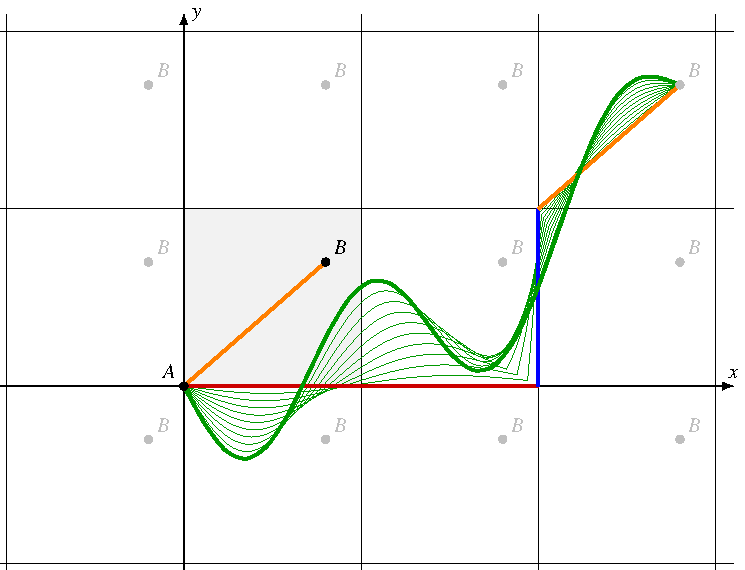
\includegraphics{chapters/120-topologie/images/toruspfade.pdf}
\caption{Ein zweidimensionaler Torus $T$ wird beschrieben als die
Punkte der zweidimensionalen Ebene, die aber als gleich betrachtet
werden, wenn sich ihre Koordinaten um eine Ganzzahl unterscheiden.
Alle Punkte $B$ in der Ebenen stellen also den gleichen Punkt auf dem
Torus dar.
Ein Weg von $A$ zu $B$ im Torus ist ein Weg von $A$ zu einem beliebigen
Repräsentanten von $B$ in der Ebene.
Jeder solche Pfad ({\color{darkgreen}grün}) kann zerlegt werden in
einen Pfad, der zunächst aus Segmenten ganzzahliger Länge parallel
zur $x$-Achse ({\color{darkred}rot}) bzw.~zur $y$-Achse
({\color{blue}blau}) besteht, gefolgt von einem Segment zum Punkt
$B$ in einem einzelnen Quadrat der Ebene ({\color{orange}orange}).
\label{buch:topologie:kohomologie:fig:toruspfade}}
\end{figure}

Der zweidimensionale Torus $T$ kann beschrieben werden als die
Menge $\mathbb{R}^2$, in der Punkte miteinander identifiziert
werden, die sich genau um $1$ in $x$- bzw.~$y$-Richtung unterscheiden.
Man definiert also eine Äquivalenzrelation $\sim$ durch
\[
(x+1,y \sim (x,y) \sim (x,y+1).
\]
Dann ist der Torus die Menge
\[
T
=
\{ (x,y) \mid x,y\in\mathbb\}
/
\sim.
\]
Diese Situation ist in
Abbildung~\ref{buch:topologie:kohomologie:fig:toruspfade}
dargestellt .

Ein zweidimensionaler Torus $T$ ist zusammenhängend, daher ist
$H^0(T)\mathbb{R}$ eindimensional.

Um die eindimensionalen Kohomologiegruppen zu berechnen, muss man
untersuchen, welche eindimensionale Kozyklen auch Koränder sind.
Sei also $\alpha\in \Omega^1(T)$ mit der Eigenschaft, dass $d\alpha=0$
ist.
Wir können $\alpha = f(x,y)\,dx + g(x,y)\,dy$ schreiben, die äussere Ableitung
ist dann
\[
d\alpha
=
\frac{\partial f}{\partial y}\,dy\wedge dx
+
\frac{\partial g}{\partial y}\,dx\wedge dy
=
\biggl(\frac{\partial g}{\partial y}-\frac{\partial f}{\partial x}\biggr)
\,dx\wedge dy.
\]
Ein Kozyklus zeichnet sich daher dadurch aus, dass
\begin{equation}
\frac{\partial g}{\partial y}-\frac{\partial f}{\partial x}
=
0
\label{buch:topologie:derham:eqn:integrabilitaet}
\end{equation}
ist.
Der Satz von Green besagt, dass unter Voraussetzung
\eqref{buch:topologie:derham:eqn:integrabilitaet}
das Wegintegral
\[
\int_\gamma \alpha
\]
für einen Weg zwischen zwei Punkten auf $\mathbb{R}^2$ nicht vom Weg
in $\mathbb{R}^2$ abhängt.

Zwei Punkte in $T$ können durch verschiedene Punkte in
$\mathbb{R}^2$ repräsentiert werden, die sich durch eine Ganzzahl
in jeder Koordinaten unterscheiden.
Zwischen den Punkten $A$ und $B$ in $T$ gibt es daher viele Wege.
In Abbildung~\ref{buch:topologie:kohomologie:fig:toruspfade} sind
mehrere Pfade dargestellt.
Der orange Pfad führt von $A=(0,0)$ zum Punkt $B$ im Einheitsquadrat.
Der grüne Pfad führt von $A=(0,0)$ zu dem weiter entfernten
Repräsentanten, dessen $x$- und $y$-Koordinaten um 2 bzw.~1 grösser
sind.
Dieser zweite Pfad kann in einen Pfad deformiert werden, der erst
zwei Einheiten lang der $x$-Achse folgt ({\color{darkred}rotes}
Teilstück), dann eine Einheit in Richtung der $y$-Achse verläuft
({\color{blue}blaues} Teilstück), um dann dem {\color{orange}orangen}
Teilstück bis zum Punkt $B$ zu folgen.

Wir wählen jetzt $A=(0,0)$ und versuchen eine Funktion $\beta$ zu
konstruieren, so dass $d\beta =\alpha$ ist.
Dazu müssen wir den Funktionswert $\beta(x,y)$ bestimmen.
Zu diesem Zweck integrieren wir über einen Weg in $T$ von $A$ nach
$B=(x,y)$, wobei wir annehmen dürfen, dass $x,y\in[0,1)$.
Jedem Weg von $A$ nach $B$ in $T$ entspricht ein Weg von $(0,0)$
zu einem Punkt $(x+k,y+l)$ in $\mathbb{R}$.
Der Weg in $T$ ist also deformierbar in einen Weg
zunächst von $(0,0)$ nach $(k,0)$ dann nach $(k,l)$ und schliesslich
zu $(x,y)$.

Wenn es die Funktion $\beta$ gibt, dann muss man sie durch Integration
entlang eines beliebigen Wegs in $T$ erhalten können.
Wie Abbildung~\ref{buch:topologie:kohomologie:fig:toruspfade}
illustriert lässt sich ein solcher Weg immer zerlegen in 
$k$ Segmente der Länge $1$ in $x$-Richtung ({\color{darkred}rot})
und $l$-Segmente der Länge $1$ in $y$-Richtunge ({\color{blue}blau})
gefolgt vom direkten Pfad im Einheitsquadrat von $(0,0)$ zu $(B)$
({\color{orange}}).
Die Funktion $\beta$ im Punkt $B$ muss daher
\begin{align*}
\beta(B)
&=
\beta(B) - \beta(A)
=
\int_{{\color{darkgreen}\gamma_{AB}}} d\beta
=
\int_{{\color{darkgreen}\gamma_{AB}}} \alpha
\\
&=
k\int_{(0,0)}^{(1,0)}\alpha
+
l\int_{(0,0)}^{(0,1)}\alpha
+
\int_{(0,0)}^{\color{orange}(B)}\alpha
\end{align*}
für beliebige $k,l\in\mathbb{Z}$.
Dies ist nur dann möglich, wenn die beiden ersten Integrale verschwinden.
Die Abbildung
\[
H^1(T)
\to
\mathbb{R}^2
:
\alpha
\mapsto
\biggl(
\int_{(0,0)}^{(1,0)}
\alpha,
\int_{(0,0)}^{(0,1)}
\alpha
\biggr)
\]
ist eine lineare Abbildung, deren Kern genau aus den Korändern besteht.
Es folgt daher, dass
\[
H^1(T) = \mathbb{R}^2
\]
zweidimensional ist.

Weiter ist $H^2(T)=\mathbb{R}$, so dass die Euler-Charakteristik des Torus
\[
\chi(T)
=
\dim H^0(T) - \dim H^1(T) + \dim H^2(T)
=
1-2+1
=
0.
\]
Dies stimmt überein mit der Euler-Charakteristik, die mit einer Triangulation
berechnet wurde.

%
% Kugel
%
\subsubsection{Kugel}
Auf einer zweidimensionalen Kugel $S^2$ sind alle Pfade zwischen zwei
Punkten ineinander deformierbar.
Für eine 1-Form $\alpha$ können wir daher die Funktion $\beta$ durch
\[
\beta(B)
=
\int_{\gamma_{AB}} \alpha
\]
definieren, wobei $\gamma_{AB}$ ein beliebiger Pfad von $A$ nach $B$.

Zwei verschiedenen Pfaden $\gamma_{AB}$ und $\tilde{\gamma}_{AB}$
lassen sich ineinander deformieren, es gibt daher eine Abbildung
\[
H
\colon
[0,1]\times[0,1] \to S^2
\qquad\text{mit}\qquad
H(t,s)
=
\begin{cases}
\gamma_{AB}(t)          &\qquad s=0\\
\tilde{\gamma}_{AB} (t) &\qquad s=1.
\end{cases}
\]
Da $H$ für $t=0$ und $t=1$ konstant ist, ist das Integral 
\begin{align*}
\int_{\gamma_{AB}} \alpha
-
\int_{\tilde{\gamma}_{AB}} \alpha
&=
\int_{\partial I^2} \alpha
=
\int_{I^2} d\alpha.
\end{align*}
Für einen Kozyklus ist $d\alpha=0$ und damit sind die beiden Wegintegrale
gleich und die Funktion $\beta$ ist wohldefiniert.
Dies zeigt, dass $\alpha=d\beta$ ein Korand ist und damit auch dass
$H^1(S^2)=0$.

Dieses Argument funktioniert natürlich für jede Mannigfaltigkeit,
in der sich jeder geschlossene Pfad zu einem Punkt zusammenziehen
lässt.
Für solche wie man sagt einfach zusammenhängenden Mannigfaltigkeiten
gilt daher $H^1(M)=0$.





